\documentclass[14pt]{extarticle}

\usepackage[table]{xcolor}
\usepackage{amsmath,mathtools,amsfonts,amsthm,amssymb,hyperref,wasysym,pifont,bm}
\usepackage{parskip,geometry,latexsym,bookmark,mathtools,float,cancel,tcolorbox}

% for the Power set P
\usepackage[mathscr]{euscript}
\let\euscr\mathscr 
\let\mathscr\relax
\usepackage[scr]{rsfso}
\newcommand{\ps}{\mathscr{P}}

\newtheorem{defn}{Definition}
\newtheorem{thm}{Theorem}
\newtheorem{claim}{Claim}
\newtheorem{lemma}{Lemma}

\renewcommand{\arraystretch}{1.3}

\newcommand{\es}{\varnothing}
\newcommand{\dps}{\displaystyle}
\newcommand{\fbl}{\underline{\hspace{1cm}}\,\,}
\newcommand{\R}{\mathbb{R}}
\newcommand{\Z}{\mathbb{Z}}
\newcommand{\from}{\leftarrow}
\newcommand{\true}{{\bf t}}
\newcommand{\false}{{\bf c}}
\newcommand{\bic}{\leftrightarrow}
\newcommand{\base}[1]{{\color{cyan}\subseteq1}}
\newcommand{\floor}[1]{{\left\lfloor\subseteq1\right\rfloor}}
\newcommand{\ceil}[1]{{\lceil\subseteq1\rceil}}
\newcommand{\da}{\downarrow}
\newcommand{\fa}{\forall}
\newcommand{\te}{\exists}
\newcommand{\cy}{\color{cyan}}

\newcommand{\colsq}[1]{{\color{\subseteq1} $\blacksquare$}}

\newcommand\Ccancel[2][black]{\renewcommand\CancelColor{\color{\subseteq1}}\cancel{\subseteq2}}
\newcommand\Cbcancel[2][black]{\renewcommand\CancelColor{\color{\subseteq1}}\bcancel{\subseteq2}}

\hypersetup{colorlinks,allcolors=blue,linktoc=all}
\geometry{a4paper}
\geometry{margin=0.42in}

\title{Chapter 6 Solutions, Susanna Epp Discrete Math 5th Edition}

\author{https://github.com/spamegg1}

\begin{document}
\maketitle
\tableofcontents

\section{Exercise Set 6.1}

\subsection{Exercise 1}
In each of (a)-(f), answer the following questions: Is \(A \subseteq B\)? Is \(B \subseteq A\)? 
Is either $A$ or $B$ a proper subset of the other?

\subsubsection{(a)}
\(A = \{2, \{2\}, (\sqrt{2})^2\}, B = \{2, \{2\}, \{\{2\}\}\}\)

\begin{proof}
\(A = \{2, \{2\}, (\sqrt{2})^2\} = \{2, \{2\}, 2\} = \{2, \{2\}\}\), so \(A \subseteq B\) because every element of $A$
is in $B$, but \(B \nsubseteq A\) because \(\{\{2\}\} \in B\) but \(\{\{2\}\} \notin A\). Thus $A$ is a proper subset of $B$.
\end{proof}

\subsubsection{(b)}
\(A = \{3, \sqrt{5^2 - 4^2}, 24 \mod 7\}, B = \{8 \mod 5\}\)

\begin{proof}
\(A = \{3, \sqrt{5^2 - 4^2}, 24 \mod 7\} = \{3, 3, 3\} = \{3\}, B = \{8 \mod 5\} = \{3\}\). So $A = B$, which means
both \(A \subseteq B\) and \(B \subseteq A\).
\end{proof}

\subsubsection{(c)}
\(A = \{\{1, 2\}, \{2, 3\}\}, B = \{1, 2, 3\}\)

\begin{proof}
\(A \nsubseteq B\) because $\{1, 2\} \in A$ but $\{1, 2\} \notin B$.
\(B \nsubseteq A\) because $1 \in B$ but $1 \notin A$.
\end{proof}

\subsubsection{(d)}
\(A = \{a, b, c\}, B = \{\{a\}, \{b\}, \{c\}\}\)

\begin{proof}
\(A \nsubseteq B\) because $a \in A$ but $a \notin B$.
\(B \nsubseteq A\) because $\{a\} \in B$ but $\{a\} \notin A$.
\end{proof}

\subsubsection{(e)}
\(A = \{\sqrt{16}, \{4\}\}, B = \{4\}\)

\begin{proof}
\(A = \{\sqrt{16}, \{4\}\} = \{4, \{4\}\}\). 
\(B \subseteq A\) because $4$ is the only element of $B$ and $4 \in A$.
\(A \nsubseteq B\) because \(\{4\} \in A\) but \(\{4\} \notin B\).
\end{proof}

\subsubsection{(f)}
\(A = \{x \in \R \, | \, \cos(x) \in \Z\}, B = \{x \in \R \, | \, \sin(x) \in \Z\}\)

\begin{proof}
From trigonometry we know that \(\cos(x)\) and \(\sin(x)\) have the only integer values $-1, 0$ and $1$. We also know that 

\(\cos(x) = -1\) if and only if \(x = \pi + 2n\pi\) for some integer $n \in \Z$ 
(\(\ldots, -3\pi, -\pi, \pi, 3\pi, \ldots\)),

\(\cos(x) = 0\) if and only if \(x = \frac{\pi}{2} + n\pi\) for some integer $n \in \Z$ 
(\(\ldots, -\frac{3\pi}{2}, -\frac{\pi}{2}, \frac{\pi}{2}, \frac{3\pi}{2}, \ldots\)),

\(\cos(x) = 1\) if and only if \(x = 2n\pi\) for some integer $n \in \Z$ 
(\(\ldots, -4\pi, -2\pi, 0, 2\pi, 4\pi, \ldots\)),

\(\sin(x) = -1\) if and only if \(x = -\frac{\pi}{2} + 2n\pi\) for some integer $n \in \Z$
(\(\ldots, -\frac{5\pi}{2}, -\frac{\pi}{2}, \frac{3\pi}{2}, \frac{7\pi}{2}, \ldots\)),

\(\sin(x) = 0\) if and only if \(x = n\pi\) for some integer $n \in \Z$,
(\(\ldots, -2\pi, -\pi, 0, \pi, 2\pi, \ldots\)),

\(\sin(x) = 1\) if and only if \(x = \frac{\pi}{2} + 2n\pi\) for some integer $n \in \Z$
(\(\ldots, -\frac{7\pi}{2}, -\frac{3\pi}{2}, \frac{\pi}{2}, \frac{5\pi}{2}, \ldots\)).

So:
\[
A = \{\cdots, -\frac{5\pi}{2}, -2\pi, -\frac{3\pi}{2}, -\pi, -\frac{\pi}{2}, 0, \frac{\pi}{2}, \pi, \frac{3\pi}{2}, 2\pi, \frac{5\pi}{2}, \cdots\}
\]
and
\[
B = \{\cdots, -\frac{5\pi}{2}, -2\pi, -\frac{3\pi}{2}, -\pi, -\frac{\pi}{2}, 0, \frac{\pi}{2}, \pi, \frac{3\pi}{2}, 2\pi, \frac{5\pi}{2}, \cdots\}
\]
so $A = B$.
\end{proof}

\subsection{Exercise 2}
Complete the proof from Example 6.1.3: 
Prove that \(B \subseteq A\) where \(A = \{m \in \Z \, | \, m = 2a \text{ for some integer } a\}\) and 
\(B = \{n \in \Z \, | \, n = 2b - 2 \text{ for some integer } b\}\)

\begin{proof}
{\bf Proof That $B \subseteq A$:} Suppose $x$ is a particular but arbitrarily chosen element of $B$. 

{\it [We must show that $x \in A$. By definition of $A$, this means we must show that $x = 2 \cdot$(some integer).]}

By definition of $B$, there is an integer $b$ such that \(x = 2b - 2\). 

{\it [Given that \(x = 2b - 2\), can $x$ also be expressed as $2 \cdot$ (some integer)? That is, is there an integer, say, a, such that \(2b - 2 = 2a\)? Solve for $a$ to obtain \(a = b - 1\). Check to see if this works.]}

Let \(a = b - 1\). 

{\it [First check that a is an integer.]} 

We know that $a$ is an integer because it is a difference of integers. 

{\it [Then check that \(x = 2a\).]}

By substitution, \(2a = 2(b - 1) = 2b - 2 = x\). Thus, by 
definition of $A$, $x$ is an element of $A$, {\it [as was to be shown]}.
\end{proof}

\subsection{Exercise 3}
Let sets $R, S$, and $T$ be defined as follows:
\begin{center}
\begin{tabular}{rcl}
$R$ & = & \(\{x \in \Z \, | \, x \text{ is divisible by 2} \}\) \\
$S$ & = & \(\{y \in \Z \, | \, y \text{ is divisible by 3} \}\) \\
$T$ & = & \(\{z \in \Z \, | \, z \text{ is divisible by 6} \}\)
\end{tabular}
\end{center}
Prove or disprove each of the following statements.

\subsubsection{(a)}
\(R \subseteq T\)

\begin{proof}
\(R \nsubseteq T\) because there are elements in $R$ that are not in $T$. For example, the number $2$ is in $R$ but 
$2$ is not in $T$ since $2$ is not divisible by $6$.
\end{proof}

\subsubsection{(b)}
\(T \subseteq R\)

\begin{proof}
\(T \subseteq R\) because every element in $T$ is in $R$ since every integer divisible by 6 is divisible by 2. To 
see why this is so, suppose $n$ is any integer that is divisible by 6. Then $n = 6m$ for some integer $m$. Since 
\(6m = 2(3m)\) and since $3m$ is an integer (being a product of integers), it follows that \(n = 2 \cdot \)(some 
integer), and, hence, that $n$ is divisible by 2.
\end{proof}

\subsubsection{(c)}
\(T \subseteq S\)

\begin{proof}
\(T \subseteq S\) because every element in $T$ is in $S$ since every integer divisible by 6 is divisible by 3. To 
see why this is so, suppose $n$ is any integer that is divisible by 6. Then $n = 6m$ for some integer $m$. Since 
\(6m = 3(2m)\) and since $2m$ is an integer (being a product of integers), it follows that \(n = 3 \cdot \)(some 
integer), and, hence, that $n$ is divisible by 3.
\end{proof}

\subsection{Exercise 4}
Let \(A = \{n \in \Z \, | \, n = 5r \text{ for some integer } r\}\) and 

\(B = \{m \in \Z \, | \, m = 20s \text{ for some integer } s\}\). Prove or disprove each of the following statements.

\subsubsection{(a)}
\(A \subseteq B\)

\begin{proof}
\(A \nsubseteq B\) because $5 \in A$ but $5 \notin B$.
\end{proof}

\subsubsection{(b)}
\(B \subseteq A\)

\begin{proof}
\(B \subseteq A\) is true. Suppose $m \in B$. Then $m = 20s$ for some integer $s$. So $m = 20s = 5(4s)$ where $4s$ 
is an integer, therefore $m \in A$.
\end{proof}

\subsection{Exercise 5}
Let \(C = \{n \in \Z \, | \, n = 6r-5 \text{ for some integer } r\}\) and \(D = \{m \in \Z \, | \, m = 3s+1 
\text{ for some integer } s\}\). Prove or disprove each of the following statements.

\subsubsection{(a)}
\(C \subseteq D\)

\begin{proof}
\(C \subseteq D\) because every element in $C$ is in $D$. To see why this is so, suppose $n$ is any element of $C$. 
Then \(n = 6r - 5\) for some integer $r$. Let \(s = 2r - 2\). Then $s$ is an integer (because products and 
differences of integers are integers), and \(3s + 1 = 3(2r - 2) + 1 = 6r - 6 + 1 = 6r - 5\), which equals $n$. Thus 
$n$ satisfies the condition for being in $D$. Hence, every element in $C$ is in $D$.
\end{proof}

\subsubsection{(b)}
\(D \subseteq C\)

\begin{proof}
\(D \nsubseteq C\) because there are elements of $D$ that are not in $C$. For example, 4 is in $D$ because 
\(4 = 3 \cdot 1 + 1\). But 4 is not in $C$ because if it were, then \(4 = 6r - 5\) for some integer $r$, which would 
imply that \(9 = 6r\), or, equivalently, that \(r = 3/2\), and this contradicts the fact that $r$ is an integer.
\end{proof}


\subsection{Exercise 6}
Let \(A = \{x \in \Z \, | \, x = 5a+2 \text{ for some integer } a\}\), 

\(B = \{y \in \Z \, | \, y = 10b-3 \text{ for some integer } b\}\) and 

\(D = \{z \in \Z \, | \, z = 10c+7 \text{ for some integer } c\}\). 
Prove or disprove each of the following statements.

\subsubsection{(a)}
\(A \subseteq B\)

\begin{proof}
\(A \nsubseteq B\) because \(2 \in A\) because \(2 = 5 \cdot 0 + 2\), but \(2 \notin B\). To see this, argue by
contradiction and assume \(2 \in B\). So \(2 = 10b - 3\) for some integer $b$. So \(5 = 10b\) and \(b = 1/2\) is an
integer, a contradiction. Therefore our supposition was false and \(2 \notin B\).
\end{proof}

\subsubsection{(b)}
\(B \subseteq A\)

\begin{proof}
Suppose \(y \in B\). Then \(y = 10b - 3\) for some integer $b$. Then \(y = 10b - 5 + 5 - 3 = 5(b-2) + 2\) where $b-2$
is an integer. Let \(a = b-2\). Therefore \(y = 5a + 2\) for some integer $a$, therefore \(y \in A\). 
This proves \(B \subseteq A\).
\end{proof}

\subsubsection{(c)}
$B = C$

\begin{proof}
{\bf Sketch of proof that \(B \subseteq C\):} If $r$ is any element of $B$ then there is an integer $b$ such that 
\(r = 10b - 3\). To show that $r$ is in $C$, you must show that there is an integer $c$ such that \(r = 10c + 7\). In 
scratch work, assume that $c$ exists and use the information that \(10b - 3\) would have to equal 
\(10c + 7\) to deduce the only possible value for $c$. Then show that this value is (1) an integer and (2) satisfies 
the equation \(r = 10c + 7\), which will allow you to conclude that $r$ is an element of $C$.

{\bf Sketch of proof that \(C \subseteq B\):} If $s$ is any element of $C$ then there is an integer $c$ such that 
\(s = 10c + 7\). To show that $s$ is in $B$, you must show that there is an integer $b$ such that \(s = 10c - 3\). In 
scratch work, assume that $b$ exists and use the information that \(10c + 7\) would have to equal 
\(10b - 3\) to deduce the only possible value for $b$. Then show that this value is (1) an integer and (2) satisfies 
the equation \(s = 10b - 3\), which will allow you to conclude that $s$ is an element of $B$.
\end{proof}

\subsection{Exercise 7}
Let \(A = \{x \in \Z \, | \, x = 6a+4 \text{ for some integer } a\}\), 

\(B = \{y \in \Z \, | \, y = 18b-2 \text{ 
for some integer } b\}\) and 

\(D = \{z \in \Z \, | \, z = 18c+16 \text{ for some integer } c\}\). 
Prove or disprove each of the following statements.

\subsubsection{(a)}
\(A \subseteq B\)

\begin{proof}
\(A \nsubseteq B\) because $10 \in A$ but $10 \notin B$. To see this, argue by contradiction and assume $10 \in B$.
Then \(10 = 18b-2\) for some integer $b$. Then \(12 = 18b\) and \(b = 12/18 = 2/3\), which is not an integer,
contradiction. Therefore our supposition was false and $10 \notin B$.
\end{proof}

\subsubsection{(b)}
\(B \subseteq A\)

\begin{proof}
Suppose $y \in B$. Then \(y = 18b-2\) for some integer $b$. Then \(y = 18b-6+6-2 = 6(3b-1) + 4\) where $3b-1$ is an 
integer. Let $a = 3b-1$. So \(y = 6a + 4\) for some integer $a$, therefore $y \in A$. This proves \(B \subseteq A\).
\end{proof}

\subsubsection{(c)}
$B = C$

\begin{proof}
Suppose $y \in B$. Then \(y = 18b-2\) for some integer $b$. Then \(y = 18b-18+18-2 = 18(b-1) + 16\) where $b-1$ is an 
integer. Let $c = b-1$. So \(y = 18c + 16\) for some integer $c$, therefore $y \in C$. This proves \(B \subseteq C\).

Suppose $z \in C$. Then \(z = 18c+16\) for some integer $c$. Then \(z = 18c+18-18+16 = 18(c+1) -2\) where $c+1$ is an integer. Let $b = c+1$. So \(z = 18b -2\) for some integer $b$, therefore $z \in B$. This proves \(C \subseteq B\).
\end{proof}

\subsection{Exercise 8}
Write in words how to read each of the following out loud. Then write each set using the symbols for union, 
intersection, set difference, or set complement.

\subsubsection{(a)}
\(\{x \in U \, | \, x \in A \text{ and } x \in B\}\)

\begin{proof}
{\it In words:} The set of all $x$ in $U$ such that $x$ is in $A$ and $x$ is in $B$.

{\it In symbolic notation:} \(A \cap B\).
\end{proof}

\subsubsection{(b)}
\(\{x \in U \, | \, x \in A \text{ or } x \in B\}\)

\begin{proof}
{\it In words:} The set of all $x$ in $U$ such that $x$ is in $A$ or $x$ is in $B$.

{\it In symbolic notation:} \(A \cup B\).
\end{proof}

\subsubsection{(c)}
\(\{x \in U \, | \, x \in A \text{ and } x \notin B\}\)

\begin{proof}
{\it In words:} The set of all $x$ in $U$ such that $x$ is in $A$ and $x$ is not in $B$.

{\it In symbolic notation:} \(A - B\).
\end{proof}

\subsubsection{(d)}
\(\{x \in U \, | \, x \notin A\}\)

\begin{proof}
{\it In words:} The set of all $x$ in $U$ such that $x$ is not in $A$.

{\it In symbolic notation:} \(A^c\).
\end{proof}

\subsection{Exercise 9}
Complete the following sentences without using the symbols \(\cup, \cap\), or $-$.

\subsubsection{(a)}
\(x \notin A \cup B\) if, and only if, \fbl.

\begin{proof}
\(x \notin A\) and \(x \notin B\)
\end{proof}

\subsubsection{(b)}
\(x \notin A \cap B\) if, and only if, \fbl.

\begin{proof}
\(x \notin A\) or \(x \notin B\)
\end{proof}

\subsubsection{(c)}
\(x \notin A - B\) if, and only if, \fbl.

\begin{proof}
\(x \notin A\) or \(x \in B\)
\end{proof}

\subsection{Exercise 10}
Let \(A = \{1, 3, 5, 7, 9\}\), \(B = \{3, 6, 9\}\), and \(C = \{2, 4, 6, 8\}\). Find each of the following:

\subsubsection{(a)}
\(A \cup B\)

\begin{proof}
\(A \cup B = \{1, 3, 5, 6, 7, 9\}\)
\end{proof}

\subsubsection{(b)}
\(A \cap B\)

\begin{proof}
\(A \cap B = \{3, 9\}\)
\end{proof}

\subsubsection{(c)}
\(A \cup C\)

\begin{proof}
\(A \cup C = \{1, 2, 3, 4, 5, 6, 7, 8, 9\}\)
\end{proof}

\subsubsection{(d)}
\(A \cap C\)

\begin{proof}
\(A \cap C = \es\)
\end{proof}

\subsubsection{(e)}
\(A - B\)

\begin{proof}
\(A - B = \{1, 5, 7\}\)
\end{proof}

\subsubsection{(f)}
\(B - A\)

\begin{proof}
\(B - A = \{6\}\)
\end{proof}

\subsubsection{(g)}
\(B \cup C\)

\begin{proof}
\(B \cup C = \{2, 3, 4, 6, 8, 9\}\)
\end{proof}

\subsubsection{(h)}
\(B \cap C\)

\begin{proof}
\(B \cap C = \{6\}\)
\end{proof}

\subsection{Exercise 11}
Let the universal set be $\R$, the set of all real numbers, and let \(A = \{x \in \R \,|\, 0 < x \leq 2\}\), \(B = \{x 
\in \R \, | \, 1 \leq x < 4\}\), and \(C = \{x \in \R \, | \, 3 \leq x < 9\}\). Find each of the following:

\subsubsection{(a)}
$A \cup B$

\begin{proof}
\(A \cup B = \{x \in \R \, | \, 0 < x < 4\}\)
\end{proof}

\subsubsection{(b)}
$A \cap B$

\begin{proof}
\(A \cap B = \{x \in \R \, | \, 1 \leq x \leq 2\}\)
\end{proof}

\subsubsection{(c)}
$A^c$

\begin{proof}
\(A^c = \{x \in \R \, | \, x \leq 0 \text{ or } 2 < x\}\)
\end{proof}

\subsubsection{(d)}
$A \cup C$

\begin{proof}
\(A \cup C = \{x \in \R \, | \, 0 < x \leq 2 \text{ or } 3 \leq x < 9\}\)
\end{proof}

\subsubsection{(e)}
$A \cap C$

\begin{proof}
$A \cap C = \es$
\end{proof}

\subsubsection{(f)}
$B^c$

\begin{proof}
\(B^c = \{x \in \R \, | \, x < 1 \text{ or } 4 \leq x\}\)
\end{proof}

\subsubsection{(g)}
$A^c \cap B^c$

\begin{proof}
\(A^c \cap B^c = \{x \in \R \, | \, x \leq 0 \text{ or } 4 \leq x\}\)
\end{proof}

\subsubsection{(h)}
$A^c \cup B^c$

\begin{proof}
\(A^c \cup B^c = \{x \in \R \, | \, x < 1 \text{ or } 2 < x\}\)
\end{proof}

\subsubsection{(i)}
$(A \cap B)^c$

\begin{proof}
\((A \cap B)^c = \{x \in \R \, | \, x < 1 \text{ or } 2 < x\}\)
\end{proof}

\subsubsection{(j)}
$(A \cup B)^c$

\begin{proof}
\((A \cup B)^c = \{x \in \R \, | \, x \leq 0 \text{ or } 4 \leq x\}\)
\end{proof}

\subsection{Exercise 12}
Let the universal set be $R$, the set of all real numbers, and let \(A = \{x \in R \,|\, -3 \leq x \leq 0\}\), \(B = 
\{x \in R \, | \, -1 < x < 2\}\), and \(C = \{x \in R \, | \, 6 < x \leq 8\}\). Find each of the following:

\subsubsection{(a)}
$A \cup B$

\begin{proof}
\(A \cup B = \{x \in \R \, | \, -3 \leq x < 2\}\)
\end{proof}

\subsubsection{(b)}
$A \cap B$

\begin{proof}
\(A \cap B = \{x \in \R \, | \, -1 < x \leq 0\}\)
\end{proof}

\subsubsection{(c)}
$A^c$

\begin{proof}
\(A^c = \{x \in \R \, | x < -3 \text{ or } 0 < x\, \}\)
\end{proof}

\subsubsection{(d)}
$A \cup C$

\begin{proof}
\(A \cup C = \{x \in \R \, | -3 \leq x \leq 0 \text{ or } 6 < x \leq 8\, \}\)
\end{proof}

\subsubsection{(e)}
$A \cap C$

\begin{proof}
\(A \cap C = \es\)
\end{proof}

\subsubsection{(f)}
$B^c$

\begin{proof}
\(B^c = \{x \in \R \, | \, x \leq -1 \text{ or } 2 \leq x\}\)
\end{proof}

\subsubsection{(g)}
$A^c \cap B^c$

\begin{proof}
\(A^c \cap B^c = \{x \in \R \, | \, x < -3 \text{ or } 2 \leq x\}\)
\end{proof}

\subsubsection{(h)}
$A^c \cup B^c$

\begin{proof}
\(A^c \cup B^c = \{x \in \R \, | \, x \leq -1 \text{ or } 0 < x\}\)
\end{proof}

\subsubsection{(i)}
$(A \cap B)^c$

\begin{proof}
\((A \cap B)^c = \{x \in \R \, | \, x \leq -1 \text{ or } 0 < x\}\)
\end{proof}

\subsubsection{(j)}
$(A \cup B)^c$

\begin{proof}
\((A \cup B)^c = \{x \in \R \, | \, x < -3 \text{ or } 2 \leq x\}\)
\end{proof}

\subsection{Exercise 13}
Let $S$ be the set of all strings of 0’s and 1’s of length 4, and let $A$ and $B$ be the following subsets of $S$: 
\(A = \{1110, 1111, 1000, 1001\}\) and \(B = \{1100, 0100, 1111, 0111\}\). Find each of the following:

\subsubsection{(a)}
$A \cap B$

\begin{proof}
\(A \cap B = \{1111\}\)
\end{proof}

\subsubsection{(b)}
$A \cup B$

\begin{proof}
\(A \cup B = \{1110, 1111, 1000, 1001, 1100, 0100, 0111\}\)
\end{proof}

\subsubsection{(c)}
$A - B$

\begin{proof}
\(A - B = \{1110, 1000, 1001\}\)
\end{proof}

\subsubsection{(d)}
$B - A$

\begin{proof}
\(B - A = \{1100, 0100, 0111\}\)
\end{proof}

\subsection{Exercise 14}
In each of the following, draw a Venn diagram for sets $A$, $B$, and $C$ that satisfy the given conditions.

\subsubsection{(a)}
\(A \subseteq B, C \subseteq B, A \cap C = \es\)

\begin{proof}
\begin{figure}[ht!]
\centering
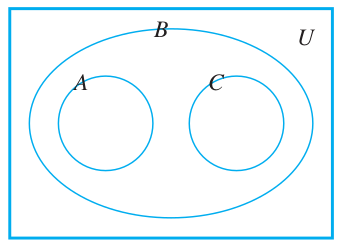
\includegraphics[scale=0.5]{../images/6.1.14.a.png}
\end{figure}
\end{proof}

\subsubsection{(b)}
\(C \subseteq A, B \cap C = \es\)

\begin{proof}
\begin{figure}[ht!]
\centering
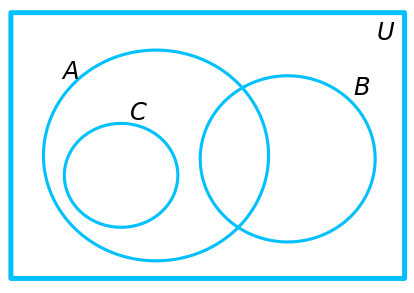
\includegraphics[scale=0.4]{../images/6.1.14.b.png}
\end{figure}
\end{proof}

\subsection{Exercise 15}
In each of the following, draw a Venn diagram for sets $A, B$, and $C$ that satisfy the given conditions.

\subsubsection{(a)}
\(A \cap B = \es, A \subseteq C, C \cap B \neq \es\)

\begin{proof}
\begin{figure}[ht!]
\centering
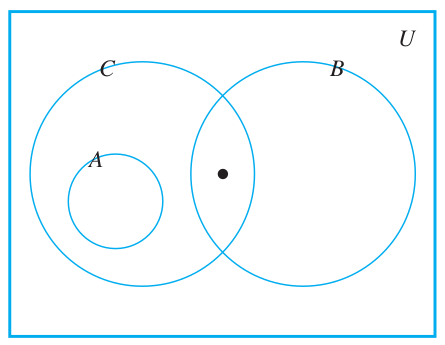
\includegraphics[scale=0.4]{../images/6.1.15.a.png}
\end{figure}
\end{proof}

\subsubsection{(b)}
\(A \subseteq B, C \subseteq B, A \cap C \neq \es\)

\begin{proof}
\begin{figure}[ht!]
\centering
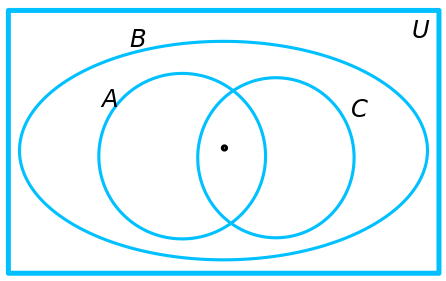
\includegraphics[scale=0.4]{../images/6.1.15.b.png}
\end{figure}
\end{proof}

\subsubsection{(c)}
\(A \cap B \neq \es, B \cap C \neq \es, A \cap C = \es, A \nsubseteq B, C \nsubseteq B\)

\begin{proof}
\begin{figure}[ht!]
\centering
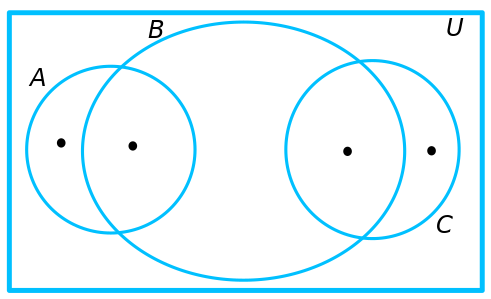
\includegraphics[scale=0.4]{../images/6.1.15.c.png}
\end{figure}
\end{proof}

\subsection{Exercise 16}
Let \(A = \{a, b, c\}, B = \{b, c, d\}, C = \{b, c, e\}\).

\subsubsection{(a)}
Find \(A \cup (B \cap C), (A \cup B) \cap C\), and \((A \cup B) \cap (A \cup C)\). Which of these sets are equal?

\begin{proof}
\(A \cup (B \cap C ) = \{a, b, c\}, (A \cup B) \cap C =
\{b, c\}\), 
and \((A \cup B) \cap (A \cup C ) = \{a, b, c, d\} \cap \{a, b, c, e\} = \{a, b, c\}\). 
Hence \(A \cup (B \cap C ) = (A \cup B) \cap (A \cup C).\)
\end{proof}

\subsubsection{(b)}
Find \(A \cap (B \cup C), (A \cap B) \cap C\), and \((A \cap B) \cup (A \cap C)\). Which of these sets are equal?

\begin{proof}
\(A \cap (B \cup C ) = \{b, c\}, (A \cap B) \cap C =
\{b, c\}\), 
and \((A \cap B) \cup (A \cap C ) = \{b, c\} \cup \{b, c\} = \{b, c\}\). 
Hence all three sets are equal.
\end{proof}

\subsubsection{(c)}
Find \((A - B) - C\) and \(A - (B - C)\). Are these sets equal?

\begin{proof}
\((A - B) - C = \{a\} - \{b, c, e\} = \{a\}\) and \(A - (B - C) = \{a, b, c\} - \{d\} = \{a, b, c\}\).
The sets are not equal.
\end{proof}

\subsection{Exercise 17}
\begin{figure}[ht!]
\centering
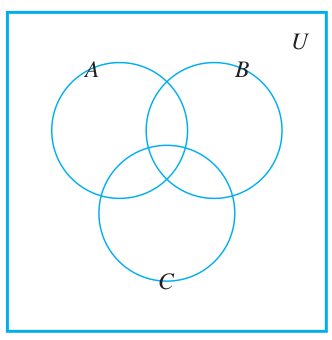
\includegraphics[scale=0.3]{../images/6.1.17.png}
\end{figure}
Consider the Venn diagram. For each of (a)-(f), copy the diagram and shade the region corresponding to the indicated set.

\subsubsection{(a)}
$A \cap B$

\begin{proof}
\begin{figure}[ht!]
\centering
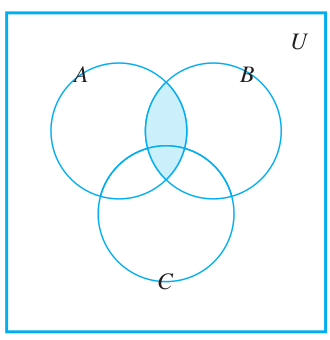
\includegraphics[scale=0.3]{../images/6.1.17.a.png}
\end{figure}
\end{proof}

\subsubsection{(b)}
$B \cup C$

\begin{proof}
\begin{figure}[ht!]
\centering
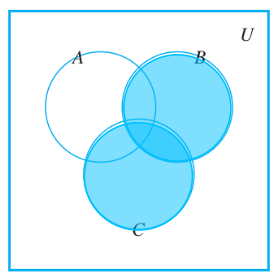
\includegraphics[scale=0.4]{../images/6.1.17.b.png}
\end{figure}
\end{proof}

\subsubsection{(c)}
$A^c$

\begin{proof}
\begin{figure}[ht!]
\centering
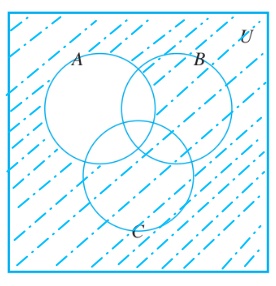
\includegraphics[scale=0.4]{../images/6.1.17.c.png}
\end{figure}
\end{proof}

\subsubsection{(d)}
$A - (B \cup C)$

\begin{proof}
\begin{figure}[ht!]
\centering
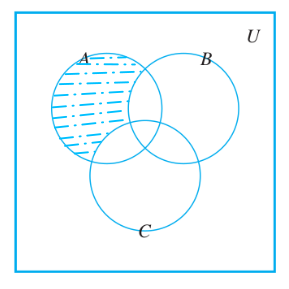
\includegraphics[scale=0.4]{../images/6.1.17.d.png}
\end{figure}
\end{proof}

\subsubsection{(e)}
$(A \cup B)^c$

\begin{proof}
\begin{figure}[ht!]
\centering
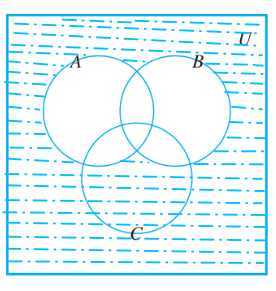
\includegraphics[scale=0.4]{../images/6.1.17.e.png}
\end{figure}
\end{proof}

\subsubsection{(f)}
$A^c \cap B^c$

\begin{proof}
Same as (e).
\end{proof}

\subsection{Exercise 18}

\subsubsection{(a)}
Is the number 0 in $\es$? Why?

\begin{proof}
The number 0 is not in $\es$ because $\es$ has no elements.
\end{proof}

\subsubsection{(b)}
Is $\es = \{\es\}$? Why?

\begin{proof}
No. The left-hand set is the empty set; it does not have any elements. The right-hand set is a set with one element, namely $\es$.
\end{proof}

\subsubsection{(c)}
Is $\es \in \{\es\}$? Why?

\begin{proof}
Yes. The left-hand side is the empty set; the right-hand side is a set with one element, namely $\es$. So the left-
hand side is an element of the right-hand side.
\end{proof}

\subsubsection{(d)}
Is $\es \in \es$? Why?

\begin{proof}
$\es$ is not in $\es$ because $\es$ has no elements.
\end{proof}

\subsection{Exercise 19}
Let \(A_i = \{i, i^2\}\) for each integer \(i = 1, 2, 3, 4\).

\subsubsection{(a)}
\(A_1 \cup A_2 \cup A_3 \cup A_4 = ?\)

\begin{proof}
\(A_1 = \{1, 1^2\} = \{1\}, A_2 = \{2, 2^2\} = \{2, 4\}, A_3 = \{3, 3^2\} = \{3, 9\}, A_4 = \{4, 4^2\} = \{4, 16\}\)

\(A_1 \cup A_2 \cup A_3 \cup A_4 = \{1\} \cup \{2, 4\} \cup \{3, 9\} \cup \{4, 16\} = \{1, 2, 3, 4, 9, 16\}\)
\end{proof}

\subsubsection{(b)}
\(A_1 \cap A_2 \cap A_3 \cap A_4 = ?\)

\begin{proof}
\(A_1 \cap A_2 \cap A_3 \cap A_4 = \{1\} \cap \{2, 4\} \cap \{3, 9\} \cap \{4, 16\} = \es\)
\end{proof}

\subsubsection{(c)}
Are \(A_1, A_2, A_3, A_4\) mutually disjoint? Explain.

\begin{proof}
\(A_1, A_2, A_3, A_4\) are not mutually disjoint, because \(A_2 \cap A_4 = \{4\} \neq \es\).
\end{proof}

\subsection{Exercise 20}
Let \(B_i = \{x \in \R \, | \, 0 \leq x \leq i\}\) for each integer \(i = 1, 2, 3, 4\).

\subsubsection{(a)}
\(B_1 \cup B_2 \cup B_3 \cup B_4 = ?\)

\begin{proof}
\(B_1 \cup B_2 \cup B_3 \cup B_4 = B_4 = [0, 4]\)
\end{proof}

\subsubsection{(b)}
\(B_1 \cap B_2 \cap B_3 \cap B_4 = ?\)

\begin{proof}
\(B_1 \cap B_2 \cap B_3 \cap B_4 = B_1 = [0, 1]\)
\end{proof}

\subsubsection{(c)}
Are \(B_1, B_2, B_3, B_4\) mutually disjoint? Explain.

\begin{proof}
No, because for example \(B_1 \cap B_2 = B_1 \neq \es\).
\end{proof}

\subsection{Exercise 21}
Let \(C_i = \{-i, i\}\) for each nonnegative integer $i$.

\subsubsection{(a)}
\(\dps \bigcup_{i=0}^{4}C_i = ?\)

\begin{proof}
\(C_0 = \{0, -0\} = \{0\}, C_1 = \{1, -1\}, C_2 = \{2, -2\}, C_3 = \{3, -3\}, C_4 = \{4, -4\}\)

\(\dps \bigcup_{i=0}^{4}C_i = \{-4, -3, -2, -1, 0, 1, 2, 3, 4\}\)
\end{proof}

\subsubsection{(b)}
\(\dps \bigcap_{i=0}^{4}C_i = ?\)

\begin{proof}
\(\dps \bigcap_{i=0}^{4}C_i = \{0\} \cap \{1, -1\} \cap \{2, -2\} \cap \{3, -3\} \cap \{4, -4\} = \es\)
\end{proof}

\subsubsection{(c)}
Are \(C_0, C_1, C_2, \ldots\) mutually disjoint? Explain.

\begin{proof}
$C_0, C_1, C_2, \ldots$ are mutually disjoint because no two of the sets have any elements in common.
\end{proof}

\subsubsection{(d)}
\(\dps \bigcup_{i=0}^{n}C_i = ?\)

\begin{proof}
\(\dps \bigcup_{i=0}^{n}C_i = \{-n, -(n-1), \ldots, -2, -1, 0, 1, 2, \ldots, n-1, n\}\)
\end{proof}

\subsubsection{(e)}
\(\dps \bigcap_{i=0}^{n}C_i = ?\)

\begin{proof}
\(\dps \bigcap_{i=0}^{n}C_i = \es\)
\end{proof}

\subsubsection{(f)}
\(\dps \bigcup_{i=0}^{\infty}C_i = ?\)

\begin{proof}
\(\dps \bigcup_{i=0}^{\infty}C_i = \Z\), the set of all integers
\end{proof}

\subsubsection{(g)}
\(\dps \bigcap_{i=0}^{\infty}C_i = ?\)

\begin{proof}
\(\dps \bigcap_{i=0}^{\infty}C_i = \es\)
\end{proof}

\subsection{Exercise 22}
Let \(D_i = \{x \in \R \,|\, -i \leq x \leq i\} = [-i, i]\) for each nonnegative integer $i$.

\subsubsection{(a)}
\(\dps \bigcup_{i=0}^{4}D_i = ?\)

\begin{proof}
\(D_0 = [-0, 0] = \{0\}, D_1 = [-1, 1], D_2 = [-2, 2], D_3 = [-3, 3], D_4 = [-4, 4]\)

\(\dps \bigcup_{i=0}^{4}D_i = \{0\} \cup [-1, 1] \cup [-2, 2] \cup [-3, 3] \cup [-4, 4] = [-4, 4]\)
\end{proof}

\subsubsection{(b)}
\(\dps \bigcap_{i=0}^{4}D_i = ?\)

\begin{proof}
\(\dps \bigcap_{i=0}^{4}D_i = \{0\} \cap [-1, 1] \cap [-2, 2] \cap [-3, 3] \cap [-4, 4] = \{0\}\)
\end{proof}

\subsubsection{(c)}
Are \(D_0, D_1, D_2, \ldots\) mutually disjoint? Explain.

\begin{proof}
$D_0, D_1, D_2, \ldots,$ are not mutually disjoint. In fact, each \(D_k \subseteq D_{k+1}\).
\end{proof}

\subsubsection{(d)}
\(\dps \bigcup_{i=0}^{n}D_i = ?\)

\begin{proof}
\(\dps \bigcup_{i=0}^{n}D_i = [-n, n]\)
\end{proof}

\subsubsection{(e)}
\(\dps \bigcap_{i=0}^{n}D_i = ?\)

\begin{proof}
\(\dps \bigcap_{i=0}^{n}D_i = \{0\}\)
\end{proof}

\subsubsection{(f)}
\(\dps \bigcup_{i=0}^{\infty}D_i = ?\)

\begin{proof}
\(\dps \bigcup_{i=0}^{\infty}D_i = \R\), the set of all real numbers
\end{proof}

\subsubsection{(g)}
\(\dps \bigcap_{i=0}^{\infty}D_i = ?\)

\begin{proof}
\(\dps \bigcap_{i=0}^{\infty}D_i = \{0\}\)
\end{proof}

\subsection{Exercise 23}
Let \(V_i = \{x \in \R \,|\, -\frac{1}{i} \leq x \leq \frac{1}{i}\} = [-\frac{1}{i}, \frac{1}{i}]\) 
for each positive integer $i$.

\subsubsection{(a)}
\(\dps \bigcup_{i=1}^{4}V_i = ?\)

\begin{proof}
\(\dps \bigcup_{i=1}^{4}V_i = V_1 = [-1, 1]\)
\end{proof}

\subsubsection{(b)}
\(\dps \bigcap_{i=1}^{4}V_i = ?\)

\begin{proof}
\(\dps \bigcap_{i=1}^{4}V_i = V_4 = \left[-\frac{1}{4}, \frac{1}{4}\right]\)
\end{proof}

\subsubsection{(c)}
Are \(V_1, V_2, V_3, \ldots\) mutually disjoint? Explain.

\begin{proof}
$V_1, V_2, V_3, \ldots,$ are not mutually disjoint. In fact, each \(V_{k+1} \subseteq V_k\).
\end{proof}

\subsubsection{(d)}
\(\dps \bigcup_{i=1}^{n}V_i = ?\)

\begin{proof}
\(\dps \bigcup_{i=1}^{n}V_i = V_1 = [-1, 1]\)
\end{proof}

\subsubsection{(e)}
\(\dps \bigcap_{i=1}^{n}V_i = ?\)

\begin{proof}
\(\dps \bigcap_{i=1}^{n}V_i = V_n = \left[-\frac{1}{n}, \frac{1}{n}\right]\)
\end{proof}

\subsubsection{(f)}
\(\dps \bigcup_{i=1}^{\infty}V_i = ?\)

\begin{proof}
\(\dps \bigcup_{i=1}^{\infty}V_i = V_1 = [-1, 1]\)
\end{proof}

\subsubsection{(g)}
\(\dps \bigcap_{i=1}^{\infty}V_i = ?\)

\begin{proof}
\(\dps \bigcap_{i=1}^{\infty}V_i = \{0\}\)
\end{proof}

\subsection{Exercise 24}
Let \(W_i = \{x \in \R \,|\, i < x\} = (i, \infty)\) for each nonnegative integer $i$.

\subsubsection{(a)}
\(\dps \bigcup_{i=0}^{4}W_i = ?\)

\begin{proof}
\(\dps \bigcup_{i=0}^{4}W_i = W_0 = (0, \infty)\)
\end{proof}

\subsubsection{(b)}
\(\dps \bigcap_{i=0}^{4}W_i = ?\)

\begin{proof}
\(\dps \bigcap_{i=0}^{4}W_i = W_4 = (4, \infty)\)
\end{proof}

\subsubsection{(c)}
Are \(W_0, W_1, W_2, \ldots\) mutually disjoint? Explain.

\begin{proof}
$W_0, W_1, W_2, \ldots,$ are not mutually disjoint. In fact, each \(W_{k+1} \subseteq W_k\).
\end{proof}

\subsubsection{(d)}
\(\dps \bigcup_{i=0}^{n}W_i = ?\)

\begin{proof}
\(\dps \bigcup_{i=0}^{n}W_i = W_0 = (0, \infty)\)
\end{proof}

\subsubsection{(e)}
\(\dps \bigcap_{i=0}^{n}W_i = ?\)

\begin{proof}
\(\dps \bigcap_{i=0}^{n}W_i = W_n = (n, \infty)\)
\end{proof}

\subsubsection{(f)}
\(\dps \bigcup_{i=0}^{\infty}W_i = ?\)

\begin{proof}
\(\dps \bigcup_{i=0}^{\infty}W_i = W_0 = (0, \infty)\)
\end{proof}

\subsubsection{(g)}
\(\dps \bigcap_{i=0}^{\infty}W_i = ?\)

\begin{proof}
\(\dps \bigcap_{i=0}^{\infty}W_i = \es\)
\end{proof}

\subsection{Exercise 25}
Let \(R_i = \{x \in \R \,|\, 1 \leq x \leq 1 + \frac{1}{i}\} = \left[1, 1 + \frac{1}{i}\right]\) 
for each positive integer $i$.

\subsubsection{(a)}
\(\dps \bigcup_{i=1}^{4}R_i = ?\)

\begin{proof}
\(\dps \bigcup_{i=1}^{4}R_i = R_1 = [1, 2]\)
\end{proof}

\subsubsection{(b)}
\(\dps \bigcap_{i=1}^{4}R_i = ?\)

\begin{proof}
\(\dps \bigcap_{i=1}^{4}R_i = R_4 = \left[1, \frac{5}{4}\right]\)
\end{proof}

\subsubsection{(c)}
Are \(R_1, R_2, R_3, \ldots\) mutually disjoint? Explain.

\begin{proof}
No, in fact each \(R_{k+1} \subseteq R_k\).
\end{proof}

\subsubsection{(d)}
\(\dps \bigcup_{i=1}^{n}R_i = ?\)

\begin{proof}
\(\dps \bigcup_{i=1}^{n}R_i = R_1 = [1, 2]\)
\end{proof}

\subsubsection{(e)}
\(\dps \bigcap_{i=1}^{n}R_i = ?\)

\begin{proof}
\(\dps \bigcap_{i=1}^{n}R_i = R_n = \left[1, 1+\frac{1}{n}\right]\)
\end{proof}

\subsubsection{(f)}
\(\dps \bigcup_{i=1}^{\infty}R_i = ?\)

\begin{proof}
\(\dps \bigcup_{i=1}^{\infty}R_i = R_1 = [1, 2]\)
\end{proof}

\subsubsection{(g)}
\(\dps \bigcap_{i=1}^{\infty}R_i = ?\)

\begin{proof}
\(\dps \bigcap_{i=1}^{\infty}R_i = \{1\}\)
\end{proof}

\subsection{Exercise 26}
Let \(S_i = \{x \in \R \,|\, 1 < x < 1 + \frac{1}{i}\} = \left(1, 1 + \frac{1}{i}\right)\) 
for each positive integer $i$.

\subsubsection{(a)}
\(\dps \bigcup_{i=1}^{4}S_i = ?\)

\begin{proof}
\(\dps \bigcup_{i=1}^{4}S_i = S_1 = (1, 2)\)
\end{proof}

\subsubsection{(b)}
\(\dps \bigcap_{i=1}^{4}S_i = ?\)

\begin{proof}
\(\dps \bigcap_{i=1}^{4}S_i = S_4 = (1, 5/4)\)
\end{proof}

\subsubsection{(c)}
Are \(S_0, S_1, S_2, \ldots\) mutually disjoint? Explain.

\begin{proof}
No, in fact each \(S_{k+1} \subseteq S_k\).
\end{proof}

\subsubsection{(d)}
\(\dps \bigcup_{i=1}^{n}S_i = ?\)

\begin{proof}
\(\dps \bigcup_{i=1}^{n}S_i = S_1 = (1, 2)\)
\end{proof}

\subsubsection{(e)}
\(\dps \bigcap_{i=1}^{n}S_i = ?\)

\begin{proof}
\(\dps \bigcap_{i=1}^{n}S_i = S_n = (1, \frac{n+1}{n})\)
\end{proof}

\subsubsection{(f)}
\(\dps \bigcup_{i=1}^{\infty}S_i = ?\)

\begin{proof}
\(\dps \bigcup_{i=1}^{\infty}S_i = S_1 = (1, 2)\)
\end{proof}

\subsubsection{(g)}
\(\dps \bigcap_{i=1}^{\infty}S_i = ?\)

\begin{proof}
\(\dps \bigcap_{i=1}^{\infty}S_i = (1, 1) = \es\)
\end{proof}

\subsection{Exercise 27}

\subsubsection{(a)}
Is \(\{\{a, d, e\}, \{b, c\}, \{d, f\}\}\) a partition of
\(\{a, b, c, d, e, f\}\)?

\begin{proof}
No. The element $d$ is in two of the sets.
\end{proof}

\subsubsection{(b)}
Is \(\{\{w, x, v\}, \{u, y, q\}, \{p, z\}\}\) a partition of \(\{p, q, u, v, w, x, y, z\}\)?

\begin{proof}
Yes.
\end{proof}

\subsubsection{(c)}
Is \(\{\{5, 4\}, \{7, 2\}, \{1, 3, 4\}, \{6, 8\}\}\) a partition of \(\{1, 2, 3, 4, 5, 6, 7, 8\}\)?

\begin{proof}
No. The element $4$ is in two of the sets.
\end{proof}

\subsubsection{(d)}
Is \(\{\{3, 7, 8\}, \{2, 9\}, \{1, 4, 5\}\}\) a partition of \(\{1, 2, 3, 4, 5, 6, 7, 8, 9\}\)?

\begin{proof}
No. None of the sets contains 6.
\end{proof}

\subsubsection{(e)}
Is \(\{\{1, 5\}, \{4, 7\}, \{2, 8, 6, 3\}\}\) a partition of \(\{1, 2, 3, 4, 5, 6, 7, 8\}\)?

\begin{proof}
Yes.
\end{proof}

\subsection{Exercise 28}
Let $E$ be the set of all even integers and $O$ the set of all odd integers. Is \(\{E, O\}\) a partition of $\Z$, the set of all integers? Explain your answer.

\begin{proof}
Yes. Every integer is either even or odd, and no integer is both even and odd.
\end{proof}

\subsection{Exercise 29}
Let $\R$ be the set of all real numbers. Is $\{R^+, R^-, \{0\}\}$ a partition of $\R$? Explain your answer.

\begin{proof}
Yes. Every real number is either positive or negative or zero, and no real number is both positive and negative, and 
zero is neither negative nor positive (so the three sets are mutually disjoint).
\end{proof}

\subsection{Exercise 30}
Let $Z$ be the set of all integers and let
\begin{center}
\begin{tabular}{rcl}
$A_1$ & = & \(\{n \in \Z \, | \, n = 4k \text{ for some integer } k\}\) \\
$A_2$ & = & \(\{n \in \Z \, | \, n = 4k + 1 \text{ for some integer } k\}\) \\
$A_3$ & = & \(\{n \in \Z \, | \, n = 4k + 2 \text{ for some integer } k\}\) \\
$A_4$ & = & \(\{n \in \Z \, | \, n = 4k + 3 \text{ for some integer } k\}\) 
\end{tabular}
\end{center}
Is \(\{A_0, A_1, A_2, A_3\}\) a partition of $\Z$? Explain your answer.

\begin{proof}
Yes. These sets are mutually disjoint, and by the quotient-remainder theorem, every integer has exactly one of the 
forms \(n = 4k\) or \(n = 4k+1\) or \(n = 4k+2\) or \(n = 4k+3\).
\end{proof}

\subsection{Exercise 31}
Suppose \(A = \{1, 2\}, B = \{2, 3\}\). Find each of the following:

\subsubsection{(a)}
\(\ps(A \cap B)\)

\begin{proof}
\(A \cap B = \{2\}\), so \(\ps(A \cap B) = \{\es, \{2\}\}\).
\end{proof}

\subsubsection{(b)}
\(\ps(A)\)

\begin{proof}
\(A = \{1, 2\}\), so \(\ps(A) = \{\es, \{1\}, \{2\}, \{1, 2\}\}\).
\end{proof}

\subsubsection{(c)}
\(\ps(A \cup B)\)

\begin{proof}
\(A \cup B = \{1, 2, 3\}\), so \(\ps(A \cup B) = \{\es, \{1\}, \{2\}, \{3\}, \{1, 2\}, \{1, 3\}, \{2, 3\}, \{1, 2, 3\}\}\).
\end{proof}

\subsubsection{(d)}
\(\ps(A \times B)\)

\begin{proof}
\(A \times B = \{(1, 2), (1, 3), (2, 2), (2, 3)\}\), so \(\ps(A\times B)=\{\es, \{(1, 2)\},\{(1, 3)\},\{(2, 2)\},\)

\(\{(2, 3)\}, \{(1, 2), (1, 3)\}, \{(1, 2), (2, 2)\}, \{(1, 2), (2, 3)\}, \{(1, 3), (2, 2)\}, \{(1, 3), (2, 3)\}, \)

\(\{(2, 2), (2, 3)\}, \{(1, 2), (1, 3), (2, 2)\}, \{(1, 2), (1, 3), (2, 3)\}, \{(1, 2), (2, 2), (2, 3)\}, \)

\(\{(1, 3), (2, 2), (2, 3)\}, \{(1, 2), (1, 3), (2, 2), (2, 3)\}\}\).
\end{proof}

\subsection{Exercise 32}

\subsubsection{(a)}
Suppose \(A = \{1\}, B = \{u, v\}\). Find \(\ps(A \times B)\).

\begin{proof}
\(\ps(A \times B) = \{\es, \{(1, u)\}, \{(1, v)\}, \{(1, u), (1, v)\}\}\)
\end{proof}

\subsubsection{(b)}
Suppose \(X = \{a, b\}, Y = \{x, y\}\). Find \(\ps(X \times Y)\).

\begin{proof}
\(X \times Y = \{(a, x), (a, y), (b, x), (b, y)\}\)

\(\ps(X \times Y) = \{\es, \{(a, x)\}, \{(a, y)\}, \{(b, x)\}, \{(b, y)\}, \{(a, x), (a, y)\}, \{(a, x), (b, x)\},\)

\(\{(a, x), (b, y)\}, \{(a, y), (b, x)\}, \{(a, y), (b, y)\}, \{(b, x), (b, y)\}, \{(a, x), (a, y), (b, x)\},\) 

\(\{(a, x), (a, y), (b, y)\}, \{(a, x), (b, x), (b, y)\}, \{(a, y), (b, x), (b, y)\},\) 

\(\{(a, x), (a, y), (b, x), (b, y)\}\}\)
\end{proof}

\subsection{Exercise 33}

\subsubsection{(a)}
Find \(\ps(\es)\).

\begin{proof}
\(\ps(\es) = \{\es\}\)
\end{proof}

\subsubsection{(b)}
Find \(\ps(\ps(\es))\).

\begin{proof}
\(\ps(\ps(\es)) = \ps(\{\es\}) = \{\es, \{\es\}\}\)
\end{proof}

\subsubsection{(c)}
Find \(\ps(\ps(\ps(\es)))\).

\begin{proof}
\(\ps(\ps(\ps(\es))) = \ps(\{\es, \{\es\}\}) = \{\es, \{\es\}, \{\{\es\}\}, \{\es, \{\es\}\}\}\)
\end{proof}

\subsection{Exercise 34}
Let \(A_1 = \{1\}, A_2 = \{u, v\}, A_3 = \{m, n\}\). Find each of the following sets:

\subsubsection{(a)}
$A_1 \cup (A_2 \times A_3)$

\begin{proof}
\(A_1 \cup (A_2 \times A_3) = \{1\} \cup \{(u, m), (u, n), (v, m), (v, n)\}\)

\(= \{1, (u, m), (u, n), (v, m), (v, n)\}\)
\end{proof}

\subsubsection{(b)}
$(A_1 \cup A_2) \times A_3$

\begin{proof}
\((A_1 \cup A_2) \times A_3 = \{1, u, v\} \times \{m, n\} = \{(1, m), (1, n), (u, m), (u, n), (v, m), (v, n)\}\)
\end{proof}

\subsection{Exercise 35}
Let \(A = \{a, b\}, B = \{1, 2\}, C = \{2, 3\}\). Find each of the following sets.

\subsubsection{(a)}
$A \times (B \cup C)$

\begin{proof}
\(A \times (B \cup C) = \{a, b\} \times \{1, 2, 3\}\ = \{(a, 1), (a, 2), (a, 3), (b, 1), (b, 2), (b, 3)\}\)
\end{proof}

\subsubsection{(b)}
$(A \times B) \cup (A \times C)$

\begin{proof}
\((A \times B) \cup (A \times C) = \{(a, 1), (a, 2), (b, 1), (b, 2), (a, 2), (a, 3), (b, 2), (b, 3)\}\) 

\(= \{(a, 1), (a, 2), (b, 1), (b, 2), (a, 3), (b, 3)\}\)
\end{proof}

\subsubsection{(c)}
$A \times (B \cap C)$

\begin{proof}
\(A \times (B \cap C) = \{a, b\} \times \{2\}\ = \{(a, 2), (b, 2)\}\)
\end{proof}

\subsubsection{(d)}
$(A \times B) \cap (A \times C)$

\begin{proof}
\((A \times B) \cap (A \times C) = \{(a, 1), (a, 2), (b, 1), (b, 2)\} \cap \{(a, 2), (a, 3), (b, 2), (b, 3)\}\) 

\(= \{(a, 2), (b, 2)\}\)
\end{proof}

\subsection{Exercise 36}
Trace the action of Algorithm 6.1.1 on the variables $i, j, found$, and $answer$ for $m = 3, n = 3$, and sets $A$ and 
$B$ represented as the arrays \(a[1] = u, a[2] = v, a[3] = w, b[1] = w, b[2] = u, b[3] = v\).

\begin{proof}
\begin{figure}[ht!]
\centering
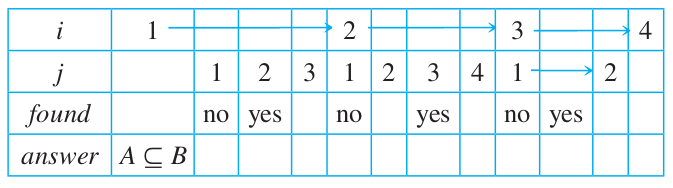
\includegraphics[scale=0.5]{../images/6.1.36.png}
\end{figure}
\end{proof}

\subsection{Exercise 37}
Trace the action of Algorithm 6.1.1 on the variables $i, j, found$, and $answer$ for $m = 4, n = 4$, and sets $A$ and 
$B$ represented as the arrays \(a[1] = u, a[2] = v, a[3] = w, a[4] = x, b[1] = r, b[2] = u, b[3] = y, b[4] = z\).

\begin{proof}
\begin{center}
\arrayrulecolor{cyan} % change rule color
\begin{tabular}{|l|c|c|c|c|c|c|c|c|}
\hline
{\bf i} & 1 & & & & 2 & & & \\
\hline
{\bf j} & 1 & 2 & 3 & 4 & 1 & 2 & 3 & 4 \\
\hline
{\bf found} & no & yes & & & no & & & \\
\hline
{\bf answer} & \(A \subseteq B\) & & & & & & & \(A \nsubseteq B\) \\
\hline
\end{tabular}
\arrayrulecolor{black} % change it back!
\end{center}
\end{proof}

\subsection{Exercise 38}
Write an algorithm to determine whether a given element $x$ belongs to a given set that is represented as the array 
\(a[1], a[2], \ldots, a[n]\).

\begin{tcolorbox}[colframe=cyan]
{\bf \cy Algorithm: Testing whether $x \in A$} 

{\bf \cy Input:} $x$ (an element), $n$ (a positive integer), \(a[1], \ldots, a[n]\) (a one-dimensional array 
representing the set $A$).

{\bf \cy Algorithm Body:}
\begin{tabbing}
\(i \coloneqq 1, answer \coloneqq\) ``\(x \notin A\)'' \\
{\bf while} \= (\(i \leq n\) and \(answer =\) ``\(x \notin A\)'') \\
            \> {\bf if} \(x = a[i]\) {\bf then} \(answer = \) ``\(x \in A\)'' \\
            \> \(i \coloneqq i + 1\) \\
{\bf end while}
\end{tabbing}
{\bf \cy Output:} {\it answer [a string]}
\end{tcolorbox}

\section{Exercise Set 6.2}
{\bf \cy Fill the blanks.}

\subsection{Exercise 1}
\subsubsection{(a)}
To say that an element is in \(A \cap (B \cup C)\) means that it is in (1) \fbl and in (2) \fbl.

\begin{proof}
(1) $A$ (2) \(B \cup C\)

\end{proof}

\subsubsection{(b)}
To say that an element is in \((A \cap B) \cup C\) means that it is in (1) \fbl or in (2) \fbl.

\begin{proof}
(1) \(A \cap B\) (2) $C$
\end{proof}

\subsubsection{(c)}
To say that an element is in \(A - (B \cap C)\) means that it is in (1) \fbl and not in (2) \fbl.

\begin{proof}
(1) $A$ (2) \(B \cap C\)
\end{proof}

\subsubsection{(d)}
To prove that \((A \cup B) \cap C \subseteq A \cup (B \cap C)\), we suppose that $x$ is any element in (1) \fbl. 
Then we must show that (2) \fbl.

\begin{proof}
(1) \((A \cup B) \cap C\) (2) \(A \cup (B \cap C)\)
\end{proof}

\subsubsection{(e)}
If $A, B$, and $C$ are any sets such that \(B \subseteq C\), to prove that \(A \cap B \subseteq A \cap C\), we 
suppose that $x$ is any element in (1) \fbl. Then we must show that (2) \fbl.

\begin{proof}
(1) \(A \cap B\) (2) \(A \cap C\)
\end{proof}

\subsection{Exercise 2}
The following are two proofs that for all sets $A$ and $B$, \(A - B \subseteq A\). The first is less formal, and the 
second is more formal. Fill in the blanks.

\subsubsection{(a)}
\underline{Proof:} Suppose $A$ and $B$ are any sets. To show that \(A - B \subseteq A\), we must show that every 
element in (1) \fbl is in (2) \fbl. But any element in \(A - B\) is in (3) \fbl and not in (4) \fbl (by definition of 
\(A - B\)). In particular, such an element is in $A$.

\begin{proof}
(1) $A - B$ (2) $A$ (3) $A$ (4) $B$
\end{proof}

\subsubsection{(b)}
\underline{Proof:} Suppose $A$ and $B$ are any sets and \(x \in A - B\). {\it [We must show that (1) \fbl.]} By 
definition of set difference, \(x \in (2)\) \fbl and \(x \notin (3)\) \fbl. In particular, \(x \in (4)\) 
{\it [which is what was to be shown].}

\begin{proof}
(1) $x \in A$ (2) $A$ (3) $B$ (4) $A$
\end{proof}

{\bf \cy In 3 and 4, supply explanations of the steps in the given proofs.}

\subsection{Exercise 3}
\underline{Theorem:} For all sets $A, B$, and $C$, if \(A \subseteq B\) and \(B \subseteq C\) then \(A \subseteq C\).

\underline{Proof:}
\begin{center}
\arrayrulecolor{cyan} % change rule color
\begin{tabular}{|l|l|}
\hline
{\bf Statement} & {\bf Explanation} \\ 
\hline
Suppose $A, B, C$ are any sets such that & starting point \\
\(A \subseteq B\) and \(B \subseteq C\). & \\
\hline
We must show that \(A \subseteq C\). & conclusion to be shown \\
\hline
Let $x$ be any element in $A$. & start of an element proof \\
\hline
Then $x$ is in $B$. & {\cy (a)} \fbl \\
\hline
It follows that $x$ is in $C$. & {\cy (b)} \fbl \\
\hline
Thus every element of $A$ is in $C$. & since $x$ could be any element of $A$ \\
\hline
Therefore \(A \subseteq C\) {\it [as was to be shown].} & {\cy (c)} \fbl \\
\hline
\end{tabular}
\arrayrulecolor{black} % change it back!
\end{center}

\begin{proof}
(a) by definition of subset (because $A \subseteq B$) (b) by definition of subset (because $B \subseteq C$) 
(c) by definition of subset
\end{proof}

\subsection{Exercise 4}
\underline{Theorem:} For all sets $A, B$, if \(A \subseteq B\) then \(A \cup B \subseteq B\).

\underline{Proof:}
\begin{center}
\arrayrulecolor{cyan} % change rule color
\begin{tabular}{|l|l|}
\hline
{\bf Statement} & {\bf Explanation} \\ 
\hline
Suppose $A, B$ are any sets such that \(A \subseteq B\). & starting point \\
\hline
We must show that \(A \cup B \subseteq B\). & conclusion to be shown \\
\hline
Let $x$ be any element in $A \cup B$. & start of an element proof \\
\hline
Then $x \in A$ or $x \in B$. & {\cy (a)} \fbl \\
\hline
In case $x \in A$, then $x \in B$. & {\cy (b)} \fbl \\
\hline
In case $x \in B$, then $x \in B$. & tautology ($p \to p)$ \\
\hline
So in either case $x \in B$. & proof by division into cases \\
\hline
Thus every element of $A \cup B$ is in $B$. & since $x$ could be any element of $A \cup B$ \\
\hline
Therefore \(A \cup B \subseteq B\) {\it [as was to be shown].} & {\cy (c)} \fbl \\
\hline
\end{tabular}
\arrayrulecolor{black} % change it back!
\end{center}

\begin{proof}
(a) by definition of union (b) by definition of subset (because \(A \subseteq B\)) (c) by definition of subset
\end{proof}

\subsection{Exercise 5}
Prove that for all sets $A$ and $B$, \((B - A) = B \cap A^c\).

\begin{proof}
Suppose $A$ and $B$ are any sets.

{\bf Proof that \(B - A \subseteq B \cap A^c\):} Suppose \(x \in B - A\). By definition of set difference, 
\(x \in B\) and \(x \notin A\). It follows by definition of complement that \(x \in B\) and \(x \in A^c\), and so by 
definition of intersection, \(x \in B \cap A^c\). {\it [Thus \(B - A \subseteq B \cap A^c\) by definition of subset.]}

{\bf Proof that \(B \cap A^c \subseteq B - A\):} Suppose \(x \in B \cap A^c\). By definition of intersection, 
\(x \in B\) and \(x \in A^c\). It follows by definition of complement that \(x \in B\) and \(x \notin A\), and so by 
definition of set difference, \(x \in B - A\). {\it [Thus \(B \cap A^c \subseteq B - A\) by definition of subset.]}

{\it [Since both subset relations have been proved, \(B - A = B \in A^c\) by definition of set equality.]}
\end{proof}

\subsection{Exercise 6}
Let $\cap$ and $\cup$ stand for the words “intersection” and “union,” respectively. Fill in the blanks in the 
following proof that for all sets $A, B$, and $C$, \(A \cap (B \cup C) = (A \cap B) \cup (A \cap C)\).

\underline{Proof:} Suppose $A$, $B$, and $C$ are any sets.

{\bf (1) Proof that \(A \cap (B \cup C) \subseteq (A \cap B) \cup (A \cap C)\):}

Let \(x \in A \cap (B \cup C)\). {\it [We must show that \(x \in {\cy (a) \fbl}\)].}

By definition of $\cup$, \(x \in {\cy (b) \fbl}\) and \(x \in B \cup C\). 
Thus \(x \in A\) and, by definition of $\cup$, \(x \in B\) or {\cy (c) \fbl}.

{\bf Case 1 (\(x \in A\) and \(x \in B\)):} In this case, \(x \in A \cap B\) by definition of $\cap$.

{\bf Case 2 (\(x \in A\) and \(x \in C\)):} In this case, \(x \in A \cap C\) by definition of $\cap$.

By cases 1 and 2, \(x \in A \cap B\) or \(x \in A \cap C\), and so, by definition of $\cup$, {\cy (d) \fbl}.

{\it [So \(A \cap (B \cup C ) \subseteq (A \cap B) \cup (A \cap C)\) by definition of subset.]}

{\bf (2) Proof that \((A \cap B) \cup (A \cap C) \subseteq A \cap (B \cup C)\):}

Let \(x \in (A \cap B) \cup (A \cap C)\). {\it [We must show that \(x \in A \cap (B \cup C )\).]}

By definition of $\cup$, \(x \in A \cap B\) {\cy (a) \fbl} \(x \in A \cap C.\)

{\bf Case 1 (\(x \in A \cap B\)):} In this case, by definition of $\cap$, \(x \in A\) and \(x \in B\). Since 
\(x \in B\), then \(x \in B \cup C\) by definition of $\cup$.

{\bf Case 2 (\(x \in A \cap C\)):} In this case, by definition of $\cap$, \(x \in A\) {\cy (b) \fbl} 
\(x \in C\). Since \(x \in C\), then \(x \in B \cup C\) by definition of $\cup$.

In both cases \(x \in A\) and \(x \in B \cup C\), and so, by definition of $\cap$, {\cy (c) \fbl}.

{\it [So \((A \cap B) \cup (A \cap C) \subseteq A \cap (B \cup C)\) by definition of {\cy (d) \fbl}.]}

{\bf (3) Conclusion:} {\it [Since both subset relations have been proved, it follows, by definition of set equality, that {\cy (a) \fbl}.]}

\begin{proof}
(1) (a) \((A \cap B) \cup (A \cap C)\) (b) $A$ (c) \(x \in C\) (d) \(x \in (A \cap B) \cup (A \cap C)\)

(2) (a) or (b) and (c) \(x \in A \cap (B \cup C)\) (d) subset

(3) (a) for all sets $A, B$, and $C$, \(A \cap (B \cup C) = (A \cap B) \cup (A \cap C)\).
\end{proof}

{\bf \cy Use an element argument to prove each statement in $7-22$. Assume that all sets are subsets of a universal set $U$.}

\subsection{Exercise 7}
For all sets $A$ and $B$, \((A \cap B)^c = A^c \cup B^c\).

\begin{proof}
Suppose $A$ and $B$ are any sets.

{\bf Proof that \((A \cap B)^c \subseteq A^c \cup B^c\):} Suppose \(x \in (A \cap B)^c\). By definition of 
complement, \(x \notin (A \cap B)\). It follows by definition of intersection that \(x \notin A\) or 
\(x \notin B\), and so by definition of complement, \(x \in A^c \) or \(x \in B^c\). So by definition of union, 
\(x \in A^c \cup B^c\). {\it [Thus \((A \cap B)^c \subseteq A^c \cup B^c\) by definition of subset.]}

{\bf Proof that \(A^c \cup B^c \subseteq (A \cap B)^c\):} Suppose \(x \in A^c \cup B^c\). By definition of union, 
\(x \in A^c\) or \(x \in B^c\). By definition of complement, \(x \notin A\) or \(x \notin B\). It follows by 
definition of intersection that \(x \notin (A \cap B)\). Then by definition of complement, \(x \in (A \cap B)^C\).
{\it [Thus \(A^c \cup B^c \subseteq (A \cap B)^c\) by definition of subset.]}

{\it [Since both subset relations have been proved, \((A \cap B)^c = A^c \cup B^c\) by definition of set equality.]}
\end{proof}

\subsection{Exercise 8}
For all sets $A$ and $B$, \((A \cap B) \cup (A \cap B^c) = A\). (This property is used in Section 9.9.)

\begin{proof}
Suppose $A$ and $B$ are any sets.

{\bf Proof that \((A \cap B) \cup (A \cap B^c) \subseteq A\):} Suppose \(x \in (A \cap B) \cup (A \cap B^c)\). 
{\it [We must show that \(x \in A\).]}

By definition of union, \(x \in A \cap B\) or \(x \in (A \cap B^c)\).

{\bf Case 1 \((x \in A \cap B)\):} In this case $x$ is in $A$ and $x$ is in $B$, and so, in particular, \(x \in A\).

{\bf Case 2 \((x \in A \cap B^c)\):} In this case $x$ is in $A$ and $x$ is not in $B$, and so, in particular, \(x \in A\).

Thus, in either case, \(x \in A\) {\it [as was to be shown].} 

So \((A \cap B) \cup (A \cap B c ) \subseteq A\) {\it [by definition of subset].}

{\bf Proof that \(A \subseteq (A \cap B) \cup (A \cap B^c )\):} Suppose \(x \in A\). {\it [We must show that 
\(x \in (A \cap B) \cup (A \cap B^c)\).]}

Either \(x \in B\) or \(x \notin B\).

{\bf Case 1 \((x \in B)\):} In this case we know that $x$ is in $A$ and we are also assuming that $x$ is in $B$. 
Hence, by definition of intersection, \(x \in A \cap B\).

{\bf Case 2 \((x \in A \cap B^c)\):} In this case we know that $x$ is in $A$ and we are also assuming that $x$ is in 
$B^c$. Hence, by definition of intersection, \(x \in A \cap B^c\).

Thus, in either case \(x \in A \cap B\) or \(x \in A \cap B^c\), and so, by definition of union, \(x \in (A \cap B) 
\cup (A \cap B^c)\) {\it [as was to be shown].} 

So \(A \subseteq (A \cap B) \cup (A \cap B^c)\) {\it [by definition of subset].}

{\bf Conclusion:} Since both subset relations have been proved it follows by definition of set equality that 
\((A \cap B) \cup (A \cap B^c) = A\).
\end{proof}

\subsection{Exercise 9}
For all sets $A$, $B$, and $C$, \((A - B) \cup (C - B) = (A \cup C) - B\).

\begin{proof}
Suppose $A$, $B$, and $C$ are any sets. 

To show that \((A - B) \cup (C - B) = (A \cup C ) - B\), we must show that \((A - B) \cup (C - B) \subseteq (A \cup C) - B\) 
and that \((A \cup C) - B \subseteq (A - B) \cup (C - B)\).

{\bf Proof that \((A - B) \cup (C - B) \subseteq (A \cup C) - B\):}

Suppose that $x$ is any element in \((A - B) \cup (C - B)\). {\it [We must show that \(x \in (A \cup C ) - B\).]} 
By definition of union, \(x \in A - B\) or \(x \in C - B\).

{\bf Case 1 (\(x \in A - B\)):} Then, by definition of set difference, \(x \in A\) and \(x \notin B\). Now because 
\(x \in A\), we have that \(x \in A \cup C\) by definition of union. Hence \(x \in A \cup C\) and \(x \notin B\), and 
so, by definition of set difference, \(x \in (A \cup C ) - B\).

{\bf Case 2 (\(x \in C - B\)):} Then, by definition of set difference, \(x \in C\) and \(x \notin B\). Now because 
\(x \in C\), we have that \(x \in A \cup C\) by definition of union. Hence \(x \in A \cup C\) and \(x \notin B\), and 
so, by definition of set difference, \(x \in (A \cup C) - B\). Thus, in both cases, \(x \in (A \cup C ) - B\) 
{\it [as was to be shown].} 

So \((A - B) \cup (C - B) \subseteq (A \cup C ) - B\) {\it [by definition of subset].}

To complete the proof that \((A - B ) \cup (C - B) = (A \cup C) - B\), you must show that 
\((A \cup C) - B \subseteq (A - B) \cup (C - B)\).
\end{proof}

\subsection{Exercise 10}
For all sets $A$, $B$, and $C$, \((A \cup B) \cap C \subseteq A \cup (B \cap C)\).

\begin{proof}
Suppose A, B, and C are any sets. We will show that \((A \cup B) \cap C \subseteq A \cup (B \cap C)\).

Suppose $x$ is any element \((A \cup B) \cap C\). By definition of intersection $x$ is in \(A \cup B\) and $x$ 
is in $C$. Then by definition of union $x$ is in $A$ or $x$ is in $B$, and in both cases $x$ is in $C$. It follows by 
definition of union that in case $x$ is in $A$ and $x$ is in $C$, then $x$ is in \(A \cup (B \cap C)\) by virtue of 
being in $A$. And in case $x$ is in \(B \cap C\), then $x$ is in \(A \cup (B \cap C)\) by virtue of being in 
\(B \cap C\). Thus in both cases $x$ is in \(A \cup (B \cap C )\), which proves that every element in \((A \cup B) \cap C\)
is in \(A \cup (B \cap C)\). Hence \((A \cup B) \cap C \subseteq A \cup (B \cap C)\) by definition of subset.
\end{proof}

\subsection{Exercise 11}
For all sets $A$, $B$, and $C$, \(A \cap (B - C) \subseteq (A \cap B) - (A \cap C)\).

\begin{proof}
Assume $A,B,C$ are any sets.

1. Assume \(x \in A \cap (B - C)\). {\it [Want to show \(x \in (A \cap B) - (A \cap C)\)].}

2. By 1 and definition of intersection, $x \in A$ and $x \in B-C$.

3. By 2 and definition of difference, $x \in A$ and $x \in B$ and $x \notin C$.

4. By 3 and definition of intersection, $x \in A \cap B$.

5. By 3 and definition of intersection, $x \notin A \cap C$.

6. By 4 and 5 and definition of difference, \(x \in (A \cap B) - (A \cap C)\).

7. By 1 and 6 and definition of subset, \(A \cap (B - C) \subseteq (A \cap B) - (A \cap C)\).
\end{proof}

\subsection{Exercise 12}
For all sets $A$, $B$, and $C$, \((A \cup B) - C \subseteq (A - C) \cup (B - C)\).

\begin{proof}
Assume $A,B,C$ are any sets.

1. Assume \(x \in (A \cup B) - C\). {\it [Want to show \(x \in (A - C) \cup (B - C)\)]}.

2. By 1 and definition of difference, \(x \in A \cup B\) and \(x \notin C\).

3. By 2 and definition of union, $x \in A$ or $x \in B$.

4. By 2, 3 and definition of difference, $x \in A-C$ or $x \in B-C$.

5. By 4 and definition of union, \(x \in (A-C) \cup (B-c)\).

6. By 1 and 5 and definition of subset, \((A \cup B) - C \subseteq (A - C) \cup (B - C)\).
\end{proof}

\subsection{Exercise 13}
For all sets $A$, $B$, and $C$, \((A - B) \cap (C - B) = (A \cap C) - B\).

\begin{proof}
Assume $A,B,C$ are any sets.

1. Assume \(x \in (A - B) \cap (C - B)\). {\it [Want to show \(x \in (A \cap C) - B\).]}

2. By 1 and definition of intersection, \(x \in A - B\) and \(x \in C - B\).

3. By 2 and definition of difference, $x \in A$ and $x \in C$ and $x \notin B$.

4. By 3 and definition of intersection, \(x \in A \cap C\).

5. By 3 and 4 and definition of difference, \(x \in (A \cap C) - B\).

6. By 1 and 5 and definition of subset, \((A - B) \cap (C - B) \subseteq (A \cap C) - B\).

{\bf Now the other direction.}

7. Assume \(x \in (A \cap C) - B\). {\it [Want to show \(x \in (A - B) \cap (C - B)\).]}

8. By 7 and definition of difference, \(x \in A \cap C\) and \(x \notin B\).

9. By 8 and definition of intersection, $x \in A$ and $x \in C$ and $x \notin B$.

10. By 9 and definition of difference, \(x \in A - B\) and \(x \in C - B\).

11. By 10 and definition of intersection, \(x \in (A - B) \cap (C - B)\).

12. By 7 and 11 and definition of subset, \((A \cap C) - B \subseteq (A - B) \cap (C - B)\).

{\bf Conclusion:} 

13. By 6, 12 and definition of set equality, \((A - B) \cap (C - B) = (A \cap C) - B\).
\end{proof}

\subsection{Exercise 14}
For all sets $A$ and $B$, \(A \cup (A \cap B) = A\).

\begin{proof}
Suppose $A$ and $B$ are any sets. We will show that \(A \cup (A \cap B) \subseteq A\). 
Suppose $x$ is any element in \(A \cup (A \cap B)\). {\it [We must show that \(x \in A\).]} By definition of union, 
\(x \in A\) or \(x \in A \cap B\). In the case where \(x \in A\), clearly \(x \in A\). In the case where 
\(x \in A \cap B\), \(x \in A\) and \(x \in B\) (by definition of intersection), and so, in particular, 
\(x \in A\). Hence, in both cases \(x \in A\) {\it [as was to be shown]}. Thus \(A \cup (A \cap B) \subseteq A\) by 
definition of subset.

To complete the proof that \(A \cup (A \cap B) = A\), you must show that \(A \subseteq A \cup (B \cap A)\).
\end{proof}

\subsection{Exercise 15}
For every set $A$, \(A \cup \es = A\).

\begin{proof}
Let $A$ be any set. {\it [We must show that \(A \cup \es = A\).]} 

{\bf Proof that \(A \cup \es \subseteq A\):} Suppose \(x \in A \cup \es\). Then \(x \in A\) or \(x \in \es\) by 
definition of union. But \(x \notin \es\) since $\es$ has no elements. Hence $x \in A$. 

{\bf Proof that \(A \subseteq A \cup \es\):} Suppose \(x \in A\). Then the statement “\(x \in A\) or \(x \in \es\)” 
is true. Hence \(x \in A \cup \es\) by definition of union. {\it [Alternatively, \(A \subseteq A \cup \es\) by the 
inclusion in union property.]}

Since \(A \cup \es \subseteq A\) and \(A \subseteq A \cup \es\), then \(A \cup \es = A\) by definition of set equality.
\end{proof}

\subsection{Exercise 16}
For all sets $A$, $B$, and $C$, if \(A \subseteq B\) then \(A \cap C \subseteq B \cap C\).

\begin{proof}
Suppose $A, B$, and $C$ are any sets such that \(A \subseteq B\). Let \(x \in A \cap C\). By definition of 
intersection, \(x \in A\) and \(x \in C\). Now since \(A \subseteq B\) and \(x \in A\), then \(x \in B\). Hence 
\(x \in B\) and \(x \in C\), and so, by definition of intersection, \(x \in B \cap C\). {\it [Thus 
\(A \cap C \subseteq B \cap C\) by definition of subset.]}
\end{proof}

\subsection{Exercise 17}
For all sets $A$, $B$, and $C$, if \(A \subseteq B\) then \(A \cup C \subseteq B \cup C\).

\begin{proof}
Assume $A,B,C$ are any sets.

1. Assume \(A \subseteq B\). {\it [Want to show \((A \cup C \subseteq B \cup C\).]}

2. Assume \(x \in A \cup C\). {\it [Want to show \(x \in B \cup C\).]}

3. By 2 and definition of union, $x \in A$ or $x \in C$.

4. {\bf Case 1 ($x \in A$):} Then by 1 and definition of subset, $x \in B$. So by definition of union, \(x \in B \cup C\).

5. {\bf Case 2 ($x \in C$):} Then by definition of union, \(x \in B \cup C\).

6. By 4 and 5, \((x \in B \cup C\).

7. By 2 and 6 and definition of subset, \((A \cup C \subseteq B \cup C\), {\it [as was to be shown.]}
\end{proof}

\subsection{Exercise 18}
For all sets $A$ and $B$, if \(A \subseteq B\) then \(B^c \subseteq A^c\).

\begin{proof}
Assume $A,B$ are any sets.

1. Assume \(A \subseteq B\). {\it [Want to show \(B^c \subseteq A^c\).]}

2. Assume \(x \in B^c\). {\it [Want to show \(x \in A^c \).]}

3. By 2 and definition of complement, $x \notin B$.

4. Argue by contradiction and assume $x \in A$. Then by 1 and definition of subset, $x \in B$, which contradicts 3.
So $x \notin A$.

5. By 4 and definition of complement, $x \in A^c$.

6. By 2 and 5 and definition of subset, \(B^c \subseteq A^c\). {\it [as was to be shown.]}
\end{proof}

\subsection{Exercise 19}
For all sets $A$, $B$, and $C$, if \(A \subseteq B\) and \(A \subseteq C\) then \(A \subseteq B \cap C\).

\begin{proof}
Assume $A,B,C$ are any sets.

1. Assume \(A \subseteq B\) and \(A \subseteq C\). {\it [Want to show \(A \subseteq B \cap C\).]}

2. Assume \(x \in A\). {\it [Want to show \(x \in B \cap C\).]}

3. By 1 and 2 and definition of subset, $x \in B$ and $x \in C$.

4. By 3 and definition of intersection, \(x \in B \cap C\).

5. By 2 and 4 and definition of subset, \(A \subseteq B \cap C\), {\it [as was to be shown.]}
\end{proof}

\subsection{Exercise 20}
For all sets $A$, $B$, and $C$, if \(A \subseteq C\) and \(B \subseteq C\) then \(A \cup B \subseteq C\).

\begin{proof}
Assume $A,B,C$ are any sets.

1. Assume \(A \subseteq C\) and \(B \subseteq C\). {\it [Want to show \(A \cup B \subseteq C\).]}

2. Assume \(x \in A \cup B\). {\it [Want to show \(x \in C\).]}

3. By 2 and definition of union, $x \in A$ or $x \in B$.

4. {\bf Case 1 ($x \in A$):} Then by 1 and 3 and definition of subset, $x \in C$.

5. {\bf Case 2 ($x \in B$):} Then by 1 and 3 and definition of subset, $x \in C$.

6. By 4 and 5, $x \in C$.

7. By 2 and 6 and definition of subset, \(A \cup B \subseteq C\), {\it [as was to be shown.]}
\end{proof}

\subsection{Exercise 21}
For all sets $A$, $B$, and $C$, \(A \times (B \cup C) = (A \times B) \cup (A \times C)\).

\begin{proof}
Suppose $A, B$, and $C$ are arbitrarily chosen sets.

\(\bm{A \times (B \cup C) \subseteq (A \times B) \cup (A \times C)}\): 

Suppose \((x, y) \in A \times (B \cup C)\). {\it [We must show that \((x, y) \in (A \times B) \cup (A \times C)\).]} 
Then \(x \in A\) and \(y \in B \cup C\). By definition of union, this means that \(y \in B\) or \(y \in C\).

{\bf Case 1 \((y \in B)\):} Then, since \(x \in A, (x, y) \in A \times B\) by definition of Cartesian product. Hence 
\((x, y) \in (A \times B) \cup (A \times C)\) by definition of union.

{\bf Case 2 \((y \in C)\):} Then, since \(x \in A, (x, y) \in A \times C\) by definition of Cartesian product. Hence 
\((x, y) \in (A \times B) \cup (A \times C)\) by definition of union.

Hence, in either case, \((x, y) \in (A \times B) \cup (A \times C)\) {\it [as was to be shown].} Thus 
\(A \times (B \cup C) \subseteq (A \times B) \cup (A \times C)\) by definition of subset.

\(\bm{(A \times B) \cup (A \times C) \subseteq A \times (B \cup C):}\) 

Suppose \((x, y) \in (A \times B) \cup (A \times C)\). Then \((x, y) \in A \times B\) or \((x, y) \in A \times C\).

{\bf Case 1 \(((x, y) \in A \times B)\):} In this case, \(x \in A\) and \(y \in B\). Now since \(y \in B\) then 
\(y \in B \cup C\) by definition of union. Hence \(x \in A\) and \(y \in B \cup C\), and so, by definition of 
Cartesian product, \((x, y) \in A \times (B \cup C)\).

{\bf Case 2 \(((x, y) \in A \times C)\):} In this case \(x \in A\) and \(y \in C\).

Now since \(y \in C\), then \(y \in B \cup C\) by definition of union. Hence \(x \in A\) and \(y \in B \cup C\), 
and so, by definition of Cartesian product, \((x, y) \in A \times (B \cup C)\). 

Thus, in either case, \((x, y) \in A \times (B \cup C)\). {\it [Hence, by definition of subset, \((A \times B) \cup (A \times C ) \subseteq A \times (B \cup C)\).]}

{\it [Since both subset relations have been proved, we can conclude that \(A \times (B \cup C) = (A \times B) \cup 
(A \times C)\) by definition of set equality.]}
\end{proof}

\subsection{Exercise 22}
For all sets $A$, $B$, and $C$, \(A \times (B \cap C) = (A \times B) \cap (A \times C)\).

\begin{proof}
Assume $A,B,C$ are any sets.

1. Assume \((x, y) \in A \times (B \cap C)\). {\it [Want to show \((x, y) \in (A \times B) \cap (A \times C)\).]}

2. By 1 and definition of Cartesian product, $x \in A$ and \(y \in B \cap C\).

3. By 2 and definition of intersection, $y \in B$ and $y \in C$.

4. By 2 and 3 and definition of Cartesian product, \((x, y) \in A \times B\) and \((x, y) \in A \times C\).

5. By 4 and definition of intersection, \((x, y) \in (A \times B) \cap (A \times C)\).

6. By 1 and 5 and definition of subset, \(A \times (B \cap C) \subseteq (A \times B) \cap (A \times C)\).

{\bf Now the reverse part:}

7. Assume \((x, y) \in (A \times B) \cap (A \times C)\). {\it [Want to show \((x, y) \in A \times (B \cap C)\).]}

8. By 7 and definition of intersection, \((x,y) \in A \times B\) and \((x,y) \in A \times C\).

9. By 8 and definition of Cartesian product, $x \in A$ and $y \in B$ and $y \in C$.

10. By 9 and definition of intersection, \(y \in B \cap C\).

11. By 9 and 10 and definition of Cartesian product, \((x,y) \in A \times (B \cap C)\).

12. By 6 and 11 and definition of subset, \((A \times B) \cap (A \times C) \subseteq A \times (B \cap C)\).

{\bf Conclusion:} By 7 and 14 and definition of set equality, \(A \times (B \cap C) = (A \times B) \cap (A \times C)\).
\end{proof}

\subsection{Exercise 23}
Find the mistake in the following “proof” that for all sets $A$, $B$, and $C$, if \(A \subseteq B\) and 
\(B \subseteq C\) then \(A \subseteq C\).

{\bf “Proof:} Suppose $A$, $B$, and $C$ are any sets such that \(A \subseteq B\) and \(B \subseteq C\). Since 
\(A \subseteq B\), there is an element $x$ such that \(x \in A\) and \(x \in B\), and since \(B \subseteq C\), there 
is an element $x$ such that \(x \in B\) and \(x \in C\). Hence there is an element $x$ such that \(x \in A\) and 
\(x \in C\) and so \(A \subseteq C\).”

\begin{proof}
There is more than one error in this “proof.” The most serious is the misuse of the definition of subset. To say 
that $A$ is a subset of B means that for every $x$, if $x \in A$ then $x \in B$. It does not mean that there exists 
an element of $A$ that is also an element of $B$. The second error in the proof occurs in the last sentence. Even 
if there is an element in $A$ that is in $B$ and an element in $B$ that is in $C$, it does not follow that there is an 
element in $A$ that is in $C$. For instance, suppose \(A = \{1, 2\}, B = \{2, 3\}\), and \(C = \{3, 4\}\). Then there 
is an element in $A$ that is in $B$ (namely 2) and there is an element in $B$ that is in $C$ (namely, 3), but there is 
no element in $A$ that is in $C$.
\end{proof}

\subsection{Exercise 24}
Find the mistake in the following “proof.”

{\bf “Theorem:”} For all sets $A$ and $B$, \(A^c \cup B^c \subseteq (A \cup B)^c\).

{\bf “Proof:} Suppose $A$ and $B$ are any sets, and \(x \in A^c \cup B^c\). Then \(x \in A^c\) or \(x \in B^c\) by 
definition of union. It follows that \(x \notin A\) or \(x \notin B\) by definition of complement, and so 
\(x \notin A \cup B\) by definition of union. Thus \(x \in (A \cup B)^c\) by definition of complement, and hence 
\(A^c \cup B^c \subseteq (A \cup B)^c\).”

{\it Hint:} The words “and so \(x \notin A \cup B\)” do not necessarily follow from “\(x \notin A\) or \(x \notin B\).” 
Try to think of an example of sets $A$ and $B$ and an element $x$ for which “\(x \notin A\) or \(x \notin B\)” is 
true and “\(x \notin A \cup B\)” is false.

\begin{proof}
(following the Hint)

Let \(A = \{x\}\) and \(B = \{y\}\). Then \(x \notin B\). So “\(x \notin A\) or \(x \notin B\)” is true. Now
\(A \cup B = \{x, y\}\) so \(x \in A \cup B\), therefore “\(x \notin A \cup B\)” is false.
\end{proof}

\subsection{Exercise 25}
Find the mistake in the following “proof” that for all sets $A$ and $B$, \((A - B) \cup (A \cap B) \subseteq A\).

{\bf “Proof:} Suppose $A$ and $B$ are any sets, and suppose \(x \in (A - B) \cup (A \cap B)\). If \(x \in A\) then 
\(x \in A - B\), and so, by definition of difference, \(x \in A\) and \(x \notin B\). In particular, \(x \in A\), 
and, therefore, \((A - B) \cup (A \cap B) \subseteq A\) by definition of subset.”

\begin{proof}
This proof has circular reasoning: it assumes what is to be proved by saying ``if $x \in A$''.

Another mistake is that ``if $x \in A$ then \(x \in A - B\)'' is an implication that does not follow. For example,
let $A = B = \{x\}$ so $x \in A$ but $A - B = \es$ thus $x \notin A - B$.
\end{proof}

\subsection{Exercise 26}
Consider the Venn diagram below.

\begin{figure}[ht!]
\centering
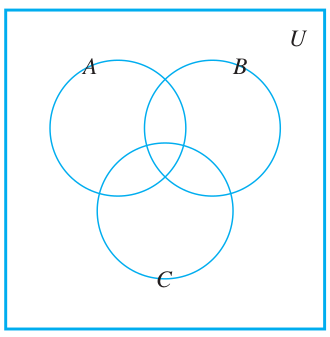
\includegraphics[scale=0.4]{../images/6.2.26.png}
\end{figure}

\subsubsection{(a)}
Illustrate one of the distributive laws by shading in the region corresponding to \(A \cup (B \cap C)\) on one copy 
of the diagram and \((A \cup B) \cap (A \cup C)\) on another.

\begin{proof}
\begin{figure}[ht!]
\centering
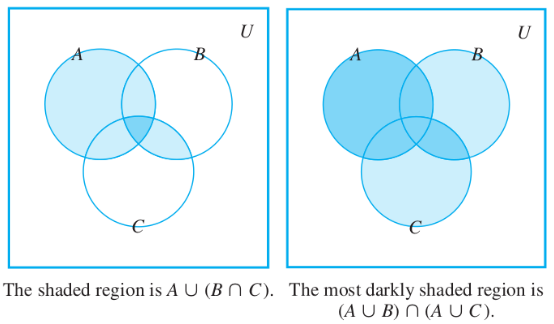
\includegraphics[scale=0.5]{../images/6.2.26.a.png}
\end{figure}
\end{proof}

\subsubsection{(b)}
Illustrate the other distributive law by shading in the region corresponding to \(A \cap (B \cup C)\) on one copy 
of the diagram and \((A \cap B) \cup (A \cap C)\) on another.

\begin{proof}
\begin{figure}[ht!]
\centering
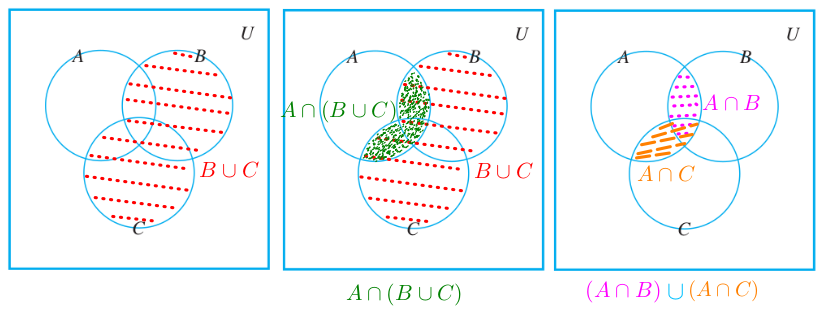
\includegraphics[scale=0.5]{../images/6.2.26.b.png}
\end{figure}
\end{proof}

\subsubsection{(c)}
Illustrate one of De Morgan’s laws by shading in the region corresponding to \((A \cup B)^c\) on one copy of the 
diagram and \(A^c \cap B^c\) on the other. (Leave the set $C$ out of your diagrams.)

\begin{proof}
\begin{figure}[ht!]
\centering
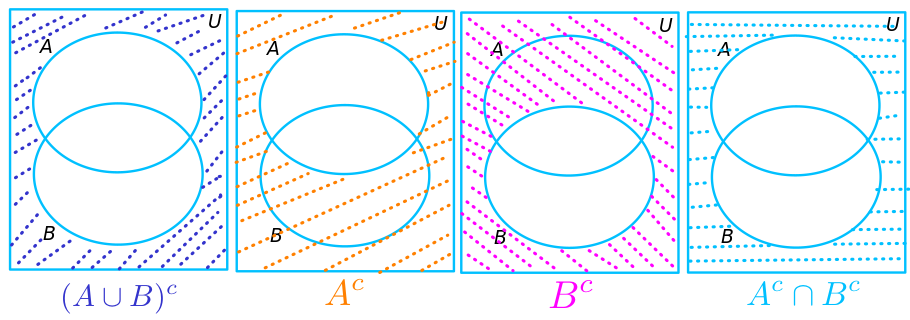
\includegraphics[scale=0.5]{../images/6.2.26.c.png}
\end{figure}
\end{proof}

\subsubsection{(d)}
Illustrate the other De Morgan’s law by shading in the region corresponding to \((A \cap B)^c\) on one copy of the 
diagram and \(A^c \cup B^c\) on the other. (Leave the set $C$ out of your diagrams.)

\begin{proof}
\begin{figure}[ht!]
\centering
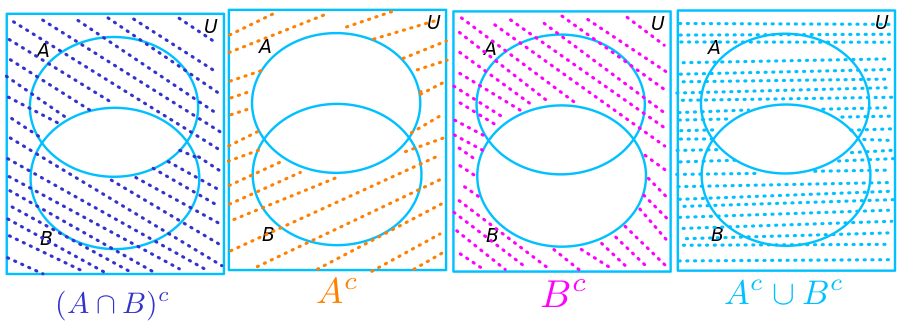
\includegraphics[scale=0.5]{../images/6.2.26.d.png}
\end{figure}
\end{proof}

\subsection{Exercise 27}
Fill in the blanks in the following proof that for all sets $A$ and $B$, \((A - B) \cap (B - A) = \es\).

\underline{Proof:} Let $A$ and $B$ be any sets and suppose \((A - B) \cap (B - A) \neq \es\). That is, suppose there 
is an element $x$ in {\cy (a) \fbl}. By definition of {\cy (b) \fbl}, \(x \in A - B\) and \(x \in {\cy (c) \fbl}\). 
Then by definition of set difference, $x \in A$ and $x \notin B$ and \(x \in {\cy (d) \fbl}\) and \(x \notin {\cy 
(e) \fbl}\). In particular $x \in A$ and \(x \notin {\cy (f) \fbl}\), which is a contradiction. Hence {\it [the 
supposition that \((A - B) \cap (B - A) \neq \es\) is false, and so]} {\cy (g) \fbl}.

\begin{proof}
(a) \((A - B) \cap (B - A)\) (b) intersection (c) $B - A$ (d) $B$ (e) $A$ (f) $A$ (g) \((A - B) \cap (B - A) = \es\)
\end{proof}

{\bf \cy Use the element method for proving a set equals the empty set to prove each statement in $28-38$. Assume that all sets are subsets of a universal set $U$.}

\subsection{Exercise 28}
For all sets $A$ and $B$, \((A \cap B) \cap (A \cap B^c) = \es)\). (This property is used in Section 9.9.)

\begin{proof}
{\it By contradiction:} Suppose not. That is, suppose there exist sets $A$ and $B$ such that \((A \cap B) \cap (A 
\cap B^c) \neq \es\). Then there is an element $x$ in \((A \cap B) \cap (A \cap B^c)\). By definition of intersection, 
\(x \in (A \cap B)\) and \(x \in (A \cap B^c)\). Applying the definition of intersection again, we have that since 
\(x \in (A \cap B), x \in A\) and \(x \in B\), and since \(x \in (A \cap B^c), x \in A\) and \(x \notin B\). Thus, in 
particular, \(x \in B\) and \(x \notin B\), which is a contradiction. It follows that the supposition is false, 
and so \((A \cap B) \cap (A \cap B^c) = \es\).
\end{proof}

\subsection{Exercise 29}
For all sets $A$, $B$, and $C$, \((A - C) \cap (B - C) \cap (A - B) = \es\).

\begin{proof}
{\it By contradiction:} Suppose not. That is, suppose there exist sets $A, B$ and $C$ such that \((A - C) \cap (B - C) 
\cap (A - B) \neq \es\). Then there is an element $x$ in \((A - C) \cap (B - C) \cap (A - B)\). By definition of 
intersection, \(x \in (A - C)\), \(x \in (B - C)\) and \(x \in (A - B)\). Applying the definition of difference, we 
have that since \(x \in (B - C), x \in B\) and \(x \notin C\), and since \(x \in (A - B), x \in A\) and \(x \notin 
B\). Thus, in particular, \(x \in B\) and \(x \notin B\), which is a contradiction. It follows that the supposition 
is false, and so \((A - C) \cap (B - C) \cap (A - B) = \es\).
\end{proof}

\subsection{Exercise 30}
For every subset $A$ of a universal set $U$, \(A \cap A^c = \es\).

\begin{proof}
Let $A$ be a subset of a universal set $U$. Suppose \(A \cap A^c \neq \es\), that is, suppose there is an element 
$x$ such that \(x \in A \cap A^c\). By definition of intersection, $x \in A$ and $x \in A^c$, and so by 
definition of complement, $x \in A$ and $x \notin A$. This is a contradiction. {\it [Hence the supposition is false, 
and we conclude that \(A \cap A^c = \es\).]}
\end{proof}

\subsection{Exercise 31}
If $U$ denotes a universal set, then \(U^c = \es\).

\begin{proof}
Suppose \(U^c \neq \es\), that is, suppose there is an element $x$ such that \(x \in U^c\). By definition of 
complement, $x \notin U$. But by definition of universal set, $x \in U$. This is a contradiction. {\it [Hence the 
supposition is false, and we conclude that \(U^c = \es\).]}
\end{proof}

\subsection{Exercise 32}
For every set $A$, \(A \times \es = \es\).

\begin{proof}
Let $A$ be a set. Suppose \(A \times \es \neq \es\). Then there would be an element $(x, y)$ in \(A \times \es\). By 
definition of Cartesian product, \(x \in A\) and \(y \in \es\). But there are no elements $y$ such that 
\(y \in \es\). Hence there are no elements \((x, y)\) in \(A \times \es\), which is a contradiction. {\it [Thus the 
supposition is false, and so \(A \times \es = \es\).]}
\end{proof}

\subsection{Exercise 33}
For all sets $A$ and $B$, if \(A \subseteq B\) then \(A \cap B^c = \es\).

\begin{proof}
Let $A$ and $B$ be sets such that \(A \subseteq B\). {\it [We must show that \(A \cap B^c = \es\).]} Suppose \(A \cap 
B^c \neq \es\); that is, suppose there were an element $x$ such that \(x \in A \cap B^c\). Then \(x \in A\) and 
\(x \in B^c\) by definition of intersection. So \(x \in A\) and \(x \notin B\) by definition of complement. But 
\(A \subseteq B\) by hypothesis, and, since \(x \in A\), then \(x \in B\) by definition of subset. Thus 
\(x \notin B\) and also \(x \in B\), which is a contradiction. Hence the supposition that \(A \cap B^c \neq 
\es\) is false, and so \(A \cap B^c = \es\).
\end{proof}

\subsection{Exercise 34}
For all sets $A$ and $B$, if \(B \subseteq A^c\) then \(A \cap B = \es\).

\begin{proof}
Let $A$ and $B$ be sets such that \(B \subseteq A^c\). {\it [We must show that \(A \cap B = \es\).]} Suppose \(A \cap B 
\neq \es\); that is, suppose there were an element $x$ such that \(x \in A \cap B\). Then \(x \in A\) and \(x \in B\) 
by definition of intersection. But \(B \subseteq A^c\) by hypothesis, and, since \(x \in B\), then \(x \in A^c\) by 
definition of subset. Thus \(x \notin A\) by definition of complement, and also \(x \in A\), which is a contradiction. 
Hence the supposition that \(A \cap B \neq \es\) is false, and so \(A \cap B = \es\).
\end{proof}

\subsection{Exercise 35}
For all sets $A$, $B$, and $C$, if \(A \subseteq B\) and \(B \cap C = \es\) then \(A \cap C = \es\).

\begin{proof}
Let $A,B$ and $C$ be sets such that \(A \subseteq B\) and \(B \cap C = \es\). {\it [We must show that \(A \cap C = 
\es\).]} Suppose \(A \cap C \neq \es\); that is, suppose there were an element $x$ such that \(x \in A \cap C\). 
Then \(x \in A\) and \(x \in C\) by definition of intersection. But \(A \subseteq B\) by hypothesis, and, 
since \(x \in A\), then \(x \in B\) by definition of subset. Thus \(x \in B\) and also \(x \in C\), so by 
definition of intersection \(x \in B \cap C\), which is a contradiction to the fact that \(B \cap C = \es\). Hence 
the supposition that \(A \cap C \neq \es\) is false, and so \(A \cap C = \es\).
\end{proof}

\subsection{Exercise 36}
For all sets $A$, $B$, and $C$, if \(C \subseteq B - A\) then \(A \cap C = \es\).

\begin{proof}
Let $A$, $B$, and $C$ be any sets such that \(C \subseteq B - A\). Suppose \(A \cap C \neq \es\). Then there is an 
element $x$ such that \(x \in A \cap C\). By definition of intersection, \(x \in A\) and \(x \in C\). Now since \(x 
\in C\) and \(C \subseteq B - A\), then \(x \in B\) and \(x \notin A\). So \(x \in A\) and \(x \notin A\), which is a 
contradiction. Hence the supposition is false, and thus \(A \cap C = \es\).
\end{proof}

\subsection{Exercise 37}
For all sets $A$, $B$, and $C$, if \(B \cap C \subseteq A\), then \((C - A) \cap (B - A) = \es\).

\begin{proof}
Let $A$, $B$, and $C$ be any sets such that \(B \cap C \subseteq A\). Suppose \((C-A) \cap (B-A) \neq \es\). Then 
there is an element $x$ such that \(x \in (C-A) \cap (B-A)\). By definition of intersection, \(x \in C-A\) and \(x 
\in B-A\). Applying the definition of difference, \(x \in C\) and \(x \notin A\), and \(x \in B\) and \(x \notin A\). 
By definition of intersection, \(x \in B \cap C\). By definition of subset, \(x \in A\). So \(x \in A\) and \(x 
\notin A\), which is a contradiction. Hence the supposition is false, and thus \((C-A) \cap (B-A) = \es\).
\end{proof}

\subsection{Exercise 38}
For all sets $A$, $B$, $C$, and $D$, if \(A \cap C = \es\) then \((A \times B) \cap (C \times D) = \es\).

\begin{proof}
Let $A, B, C$ and $D$ be any sets such that \(A \cap C = \es\). Suppose \((A \times B) \cap (C \times D) \neq \es\). 
Then there is an element $(x, y)$ such that \((x,y) \in (A \times B) \cap (C \times D)\). By definition of 
intersection, \((x,y) \in A \times B\) and \((x,y) \in C \times D\). By definition of Cartesian product, \(x \in A\) 
and \(x \in C\). By definition of intersection, \(x \in A \cap C\), which is a contradiction to the fact that \(A 
\cap C = \es\). Hence the supposition is false, and thus \((A \times B) \cap (C \times D) = \es\).
\end{proof}

{\bf \cy Prove each statement in $39-44$.}

\subsection{Exercise 39}
For all sets $A$ and $B$,

\subsubsection{(a)}
\((A - B) \cup (B - A) \cup (A \cap B) = A \cup B\)

\begin{proof}
Start of proof that \(A \cup B \subseteq (A-B) \cup (B-A) \cup (A \cap B)\): 

Given any element $x$ in \(A \cup B\), by definition of union $x$ is in at least one of $A$ and $B$. Thus $x$ 
satisfies exactly one of the following three conditions: 

(1) \(x \in A\) and \(x \notin B\) ($x$ is in $A$ only) 

(2) \(x \in B\) and \(x \notin A\) ($x$ is in $B$ only) 

(3) \(x \in A\) and \(x \in B\) ($x$ is in both $A$ and $B$)
\end{proof}

\subsubsection{(b)}
The sets \((A - B), (B - A), (A \cap B)\) are mutually disjoint.

\begin{proof}
To show that \((A - B), (B - A)\), and \((A \cap B)\) are mutually disjoint, we must show that the intersection of 
any two of them is the empty set. Now, by definition of set difference and set intersection, 

saying that \(x \in A - B\) means that (1) \(x \in A\) and \(x \notin B\), 

saying that \(x \in B - A\) means that (2) \(x \in B\) and \(x \notin A\), and 

saying that \(x \in A \cap B\) means that (3) \(x \in A\) and \(x \in B\). 

Conditions (1)–(3) are mutually exclusive: no two of them can be satisfied at the same time. Thus no element can be 
in the intersection of any two of the sets, and, therefore, the intersection of any two of the sets is the empty set. 

Hence, \((A - B), (B - A)\), and \((A \cap B)\) are mutually disjoint.
\end{proof}

\subsection{Exercise 40}
For every positive integer $n$, if $A$ and \(B_1, B_2, B_3, \ldots\) are any sets, then
\[
A \cap \left(\bigcup_{i=1}^n B_i\right) = \bigcup_{i=1}^n (A \cap B_i).
\]
\begin{proof}
Suppose that $n$ is any positive integer and that $A$ and \(B_1, B_2, B_3, \ldots\) are any sets.

{\bf Proof that} \(\bm{A \cap \left(\bigcup_{i=1}^n B_i\right) \subseteq \bigcup_{i=1}^n (A \cap B_i):}\) 

Suppose $x$ is any element in \(\dps A \cap \left( \bigcup_{i=1}^n B_i\right)\). 
{\it [We must show that \(\dps x \in \bigcup_{i=1}^n (A \cap B_i)\).]}

By definition of intersection, $x \in A$ and \(\dps x \in \bigcup_{i=1}^n B_i\). Since \(\dps x \in \bigcup_{i=1}^n 
B_i\), the definition of general union implies that \(x \in B_i\) for some \(i = 1, 2, \ldots, n\), and so, since \(x 
\in A\), the definition of intersection implies that \(x \in A \cap B_i\). Thus, by definition of general union, 
\(\dps x \in \bigcup_{i=1}^n (A \cap B_i)\) {\it [as was to be shown]}.

{\bf Proof that} \(\bm{\bigcup_{i=1}^n (A \cap B_i) \subseteq A \cap \left(\bigcup_{i=1}^n B_i\right):}\) 

Suppose $x$ is any element in \(\dps \bigcup_{i=1}^n (A \cap B_i)\). 
{\it [We must show that \(\dps x \in A \cap \left( \bigcup_{i=1}^n B_i\right)\).]}

By definition of general union, \(x \in A \cap B_i\) for some \(i = 1, 2, \ldots, n\). Thus, by definition of 
intersection, \(x \in A\) and \(x \in B_i\). Since \(x \in B_i\) for some \(i = 1, 2, \ldots, n\), then by definition 
of general union, \(\dps x \in \bigcup_{i=1}^n B_i\). Thus we have that \(x \in A\) and \(\dps x \in \bigcup_{i=1}^n 
B_i\), and so, by definition of intersection, \(\dps x \in A \cap \bigcup_{i=1}^n B_i\), {\it [as was to be shown].} 

{\bf Conclusion:} Since both subset relations have been proved, it follows by definition of set equality that 
\[
A \cap \left(\bigcup_{i=1}^n B_i\right) = \bigcup_{i=1}^n (A \cap B_i).
\]
\end{proof}

\subsection{Exercise 41}
For every positive integer $n$, if \(A_1, A_2, A_3, \ldots\) and $B$ are any sets, then
\[
\bigcup_{i=1}^n (A_i - B) = \left(\bigcup_{i=1}^n A_i\right) - B.
\]
\begin{proof}
Assume $n$ is a positive integer, \(A_1, A_2, A_3, \ldots\) and $B$ are any sets.

1. Assume \(\dps x \in \bigcup_{i=1}^n (A_i - B)\). {\it [Want to show \(\dps x \in \left(\bigcup_{i=1}^n A_i\right) - B\)].}

2. By 1 and definition of \(\dps \bigcup\), there exists a $j$ in \(\{1, \ldots, n\}\) such that \(x \in A_j - B\).

3. By 2 and definition of difference, \(x \in A_j\) and \(x \notin B\).

4. By 3 and definition of $\dps \bigcup$, \(\dps x \in \bigcup_{i=1}^n A_i\).

5. By 3 and 4 and definition of difference, \(\dps x \in \left(\bigcup_{i=1}^n A_i\right) - B\).

6. By 1 and 5 and definition of subset, \(\dps \bigcup_ {i=1}^n (A_i - B) \subseteq \left(\bigcup_{i=1}^n A_i\right) - B.\)

{\bf Now the reverse part:}

7. Assume \(\dps x \in \left(\bigcup_{i=1}^n A_i\right) - B\). {\it [Want to show \(\dps x \in \bigcup_{i=1}^n (A_i - B)\)].}

8. By 7 and definition of difference, \(\dps x \in \bigcup_{i=1}^n A_i\) and \(x \notin B\).

9. By 8 and definition of $\dps \bigcup$, there exists $j$ in \(\{1, \ldots, n\}\) such that \(x \in A_j\).

10. By 8 and 9 and definition of difference, \(x \in A_j - B\).

11. By 10 and definition of $\dps \bigcup$, \(x \in \dps \bigcup_{i=1}^n (A_i - B)\).

12. By 11 and 7 and definition of subset, \(\dps \left( \bigcup_{i=1}^n A_i\right) - B \subseteq \bigcup_{i=1}^n (A_i - B)\).

{\bf 13. Conclusion:} By 6 and 12 and definition of set equality,
\[
\bigcup_{i=1}^n (A_i - B) = \left(\bigcup_{i=1}^n A_i\right) - B.
\] 
\end{proof}

\subsection{Exercise 42}
For every positive integer $n$, if \(A_1, A_2, A_3, \ldots\) and $B$ are any sets, then
\[
\bigcap_{i=1}^n (A_i - B) = \left(\bigcap_{i=1}^n A_i\right) - B.
\]
\begin{proof}
Assume $n$ is a positive integer, \(A_1, A_2, A_3, \ldots\) and $B$ are any sets.

1. Assume \(\dps x \in \bigcap_{i=1}^n (A_i - B)\). {\it [Want to show \(\dps x \in \left(\bigcap_{i=1}^n A_i\right) - B\)].}

2. By 1 and definition of \(\dps \bigcap\), \(x \in A_i - B\) for all $i$ in \(\{1, \ldots, n\}\).

3. By 2 and definition of difference, \(x \in A_i\) for all $i$ in \(\{1, \ldots, n\}\), and \(x \notin B\).

4. By 3 and definition of $\dps \bigcap$, \(\dps x \in \bigcap_{i=1}^n A_i\).

5. By 3 and 4 and definition of difference, \(\dps x \in \left(\bigcap_{i=1}^n A_i\right) - B\).

6. By 1 and 5 and definition of subset, \(\dps \bigcap_ {i=1}^n (A_i - B) \subseteq \left(\bigcap_{i=1}^n A_i\right) - B.\)

{\bf Now the reverse part:}

7. Assume \(\dps x \in \left(\bigcap_{i=1}^n A_i\right) - B\). {\it [Want to show \(\dps x \in \bigcap_{i=1}^n (A_i - B)\)].}

8. By 7 and definition of difference, \(\dps x \in \bigcap_{i=1}^n A_i\) and \(x \notin B\).

9. By 8 and definition of $\dps \bigcap$, \(x \in A_i\) for all $i$ in \(\{1, \ldots, n\}\).

10. By 8 and 9 and definition of difference, \(x \in A_i - B\) for all $i$ in \(\{1, \ldots, n\}\).

11. By 10 and definition of $\dps \bigcap$, \(x \in \dps \bigcap_{i=1}^n (A_i - B)\).

12. By 11 and 7 and definition of subset, \(\dps \left( \bigcap_{i=1}^n A_i\right) - B \subseteq \bigcap_{i=1}^n (A_i - B)\).

{\bf 13. Conclusion:} By 6 and 12 and definition of set equality,
\[
\bigcap_{i=1}^n (A_i - B) = \left(\bigcap_{i=1}^n A_i\right) - B.
\]
\end{proof}

\subsection{Exercise 43}
For every positive integer $n$, if $A$ and \(B_1, B_2, B_3, \ldots\) are any sets, then
\[
\bigcup_{i=1}^n (A \times B_i) = A \times \left( \bigcup_{i=1}^n B_i\right).
\]
\begin{proof}
Assume $n$ is a positive integer, \(B_1, B_2, B_3, \ldots\) and $A$ are any sets.

1. Assume \(\dps (x,y) \in \bigcup_{i=1}^n (A \times B_i)\). {\it [Want to show \(\dps (x,y) \in A \times \left( 
\bigcup_{i=1}^n B_i\right)\)].}

2. By 1 and definition of \(\dps \bigcup\), there exists a $j$ in \(\{1, \ldots, n\}\) such that \((x,y) \in A \times B_j\).

3. By 2 and definition of Cartesian product, \(x \in A\) and \(y \in B_j\).

4. By 3 and definition of $\dps \bigcup$, \(\dps y \in \bigcup_{i=1}^n B_i\).

5. By 3 and 4 and definition of Cartesian product, \(\dps (x,y) \in A \times \left(\bigcup_{i=1}^n B_i\right)\).

6. By 1 and 5 and definition of subset, \(\dps \bigcup_ {i=1}^n (A \times B_i) \subseteq A \times \left(
\bigcup_{i=1}^n B_i\right).\)

{\bf Now the reverse part:}

7. Assume \(\dps (x,y) \in A \times \left(\bigcup_{i=1}^n B_i\right)\). 
{\it [Want to show \(\dps (x,y) \in \bigcup_{i=1}^n (A \times B_i)\)].}

8. By 7 and definition of Cartesian product, \(x \in A \) and \(\dps y \in \bigcup_{i=1}^n B_i\).

9. By 8 and definition of $\dps \bigcup$, there exists $j$ in \(\{1, \ldots, n\}\) such that \(y \in B_j\).

10. By 8 and 9 and definition of Cartesian product, \((x,y) \in A \times B_j\).

11. By 10 and definition of $\dps \bigcup$, \((x, y) \in \dps \bigcup_{i=1}^n (A \times B_i)\).

12. By 11 and 7 and definition of subset, \(\dps A \times \left(\bigcup_{i=1}^n B_i\right) \subseteq \bigcup_{i=1}^n (A \times B_i)\).

{\bf 13. Conclusion:} By 6 and 12 and definition of set equality,
\[
A \times \left(\bigcup_{i=1}^n B_i\right) = \bigcup_{i=1}^n (A \times B_i).
\]
\end{proof}

\subsection{Exercise 44}
For every positive integer $n$, if $A$ and \(B_1, B_2, B_3, \ldots\) are any sets, then
\[
\bigcap_{i=1}^n (A \times B_i) = A \times \left( \bigcap_{i=1}^n B_i\right).
\]
\begin{proof}
Assume $n$ is a positive integer, \(B_1, B_2, B_3, \ldots\) and $A$ are any sets.

1. Assume \(\dps (x,y) \in \bigcap_{i=1}^n (A \times B_i)\). 
{\it [Want to show \(\dps (x,y) \in A \times \left(\bigcap _{i=1}^n B_i\right)\)].}

2. By 1 and definition of \(\dps \bigcap\), \((x,y) \in A \times B_i\) for all $i$ in \(\{1, \ldots, n\}\).

3. By 2 and definition of Cartesian product, \(x \in A\) and \(y \in B_i\) for all $i$ in \(\{1, \ldots, n\}\).

4. By 3 and definition of $\dps \bigcap$, \(\dps y \in \bigcap_{i=1}^n B_i\).

5. By 3 and 4 and definition of Cartesian product, \(\dps (x, y) \in A \times \left(\bigcap_{i=1}^n B_i\right)\).

6. By 1 and 5 and definition of subset, \(\dps \bigcap _{i=1}^n (A \times B_i) \subseteq A \times \left(
\bigcap _{i=1}^n B_i\right).\)

{\bf Now the reverse part:}

7. Assume \(\dps (x,y) \in A \times \left( \bigcap_{i=1}^n B_i\right)\). {\it [Want to show \(\dps x \in \bigcap _{i=1}^n (A \times B_i)\)].}

8. By 7 and definition of Cartesian product, \(x \in A\) and \(\dps y \in \bigcap_{i=1}^n B_i\).

9. By 8 and definition of $\dps \bigcap$, \(y \in B_i\) for all $i$ in \(\{1, \ldots, n\}\).

10. By 8 and 9 and definition of Cartesian product, \((x,y) \in A \times B_i\) for all $i$ in \(\{1, \ldots, n\}\).

11. By 10 and definition of $\dps \bigcap$, \((x,y) \in \dps \bigcap_{i=1}^n (A \times B_i)\).

12. By 11 and 7 and definition of subset, \(\dps A \times \left(\bigcap_{i=1}^n B_i\right) \subseteq \bigcap_{i=1}^n 
(A \times B_i)\).

{\bf 13. Conclusion:} By 6 and 12 and definition of set equality,
\[
\bigcap_{i=1}^n (A \times B_i) = A \times \left( \bigcap_{i=1}^n B_i\right).
\]
\end{proof}

\end{document}
